% Impala Operating System
%
% Copyright (C) 2009 University of Wroclaw. Department of Computer Science
%    http://www.ii.uni.wroc.pl/
% Copyright (C) 2009 Mateusz Kocielski, Artur Koninski, Pawel Wieczorek
%    http://trzask.codepainters.com/impala/trac/
% All rights reserved.
%
% Redistribution and use in source and binary forms, with or without
% modification, are permitted provided that the following conditions
% are met:
% 1. Redistributions of source code must retain the above copyright
%  notice, this list of conditions and the following disclaimer.
% 2. Redistributions in binary form must reproduce the above copyright
%  notice, this list of conditions and the following disclaimer in the
%  documentation and/or other materials provided with the distribution.
%
% THIS SOFTWARE IS PROVIDED BY AUTHOR AND CONTRIBUTORS ``AS IS'' AND
% ANY EXPRESS OR IMPLIED WARRANTIES, INCLUDING, BUT NOT LIMITED TO, THE
% IMPLIED WARRANTIES OF MERCHANTABILITY AND FITNESS FOR A PARTICULAR PURPOSE
% ARE DISCLAIMED.  IN NO EVENT SHALL AUTHOR OR CONTRIBUTORS BE LIABLE
% FOR ANY DIRECT, INDIRECT, INCIDENTAL, SPECIAL, EXEMPLARY, OR CONSEQUENTIAL
% DAMAGES (INCLUDING, BUT NOT LIMITED TO, PROCUREMENT OF SUBSTITUTE GOODS
% OR SERVICES; LOSS OF USE, DATA, OR PROFITS; OR BUSINESS INTERRUPTION)
% HOWEVER CAUSED AND ON ANY THEORY OF LIABILITY, WHETHER IN CONTRACT, STRICT
% LIABILITY, OR TORT (INCLUDING NEGLIGENCE OR OTHERWISE) ARISING IN ANY WAY
% OUT OF THE USE OF THIS SOFTWARE, EVEN IF ADVISED OF THE POSSIBILITY OF
% SUCH DAMAGE.
%
% $Id$


\documentclass[a4paper,11pt]{report}
\usepackage{fix-cm}
\usepackage{polski}
\usepackage[latin2]{inputenc}
\usepackage{a4wide}
\usepackage{graphicx}

\author{
    Artur Koni�ski &
    Mateusz Kocielski \\
    \multicolumn{2}{c}{Pawe� Wieczorek}
}

\title{System operacyjny Impala.\\
\small{Dokumentacja projektu licencjackiego na Uniwersytecie Wroc�awskim.}
}

\makeatletter
\renewcommand\maketitle{
\begin{titlepage}

\vspace{4cm} 
{\LARGE \centering \scshape
	\begin{tabular}{cc}
		\@author
	\end{tabular}
\par}
\vspace{3cm}
{ \centering \scshape \fontsize{44}{50}\selectfont
	System operacyjny Impala\par
}
\hrulefill
\begin{flushright} { \large \scshape
Licencjacki projekt programistyczny\\ \vspace{0.20cm}
Uniwersytet Wroc�awski\\ \vspace{0.20cm}
\par
}
\end{flushright}
\end{titlepage}}
\makeatother

\begin{document}

\maketitle

\tableofcontents

% Impala Operating System
%
% Copyright (C) 2009 University of Wroclaw. Department of Computer Science
%    http://www.ii.uni.wroc.pl/
% Copyright (C) 2009 Mateusz Kocielski, Artur Koninski, Pawel Wieczorek
%    http://trzask.codepainters.com/impala/trac/
% All rights reserved.
%
% Redistribution and use in source and binary forms, with or without
% modification, are permitted provided that the following conditions
% are met:
% 1. Redistributions of source code must retain the above copyright
%  notice, this list of conditions and the following disclaimer.
% 2. Redistributions in binary form must reproduce the above copyright
%  notice, this list of conditions and the following disclaimer in the
%  documentation and/or other materials provided with the distribution.
%
% THIS SOFTWARE IS PROVIDED BY AUTHOR AND CONTRIBUTORS ``AS IS'' AND
% ANY EXPRESS OR IMPLIED WARRANTIES, INCLUDING, BUT NOT LIMITED TO, THE
% IMPLIED WARRANTIES OF MERCHANTABILITY AND FITNESS FOR A PARTICULAR PURPOSE
% ARE DISCLAIMED.  IN NO EVENT SHALL AUTHOR OR CONTRIBUTORS BE LIABLE
% FOR ANY DIRECT, INDIRECT, INCIDENTAL, SPECIAL, EXEMPLARY, OR CONSEQUENTIAL
% DAMAGES (INCLUDING, BUT NOT LIMITED TO, PROCUREMENT OF SUBSTITUTE GOODS
% OR SERVICES; LOSS OF USE, DATA, OR PROFITS; OR BUSINESS INTERRUPTION)
% HOWEVER CAUSED AND ON ANY THEORY OF LIABILITY, WHETHER IN CONTRACT, STRICT
% LIABILITY, OR TORT (INCLUDING NEGLIGENCE OR OTHERWISE) ARISING IN ANY WAY
% OUT OF THE USE OF THIS SOFTWARE, EVEN IF ADVISED OF THE POSSIBILITY OF
% SUCH DAMAGE.
%
% $Id$

\chapter{Opis projektu.}

\section{Wst�p.}

System operacyjny Impala zosta� zrealizowany w~ramach licencjackiego
projektu programistycznego na~Uniwersytecie Wroc�awskim. W~sk�ad
systemu wchodzi j�dro, biblioteka systemowa (j�zyka C), biblioteka w�tk�w
oraz oprogramowanie. System jest wzorowany na~systemach wywodz�cych si�
z~systemu UNIX i~przeznaczony jest dla~komputer�w klasy PC. 

\subsection{Cele i motywacje projektu.}

G��wnym celem i~motywacj� do~powstania projektu by�a ch�� stworzenia systemu
operacyjnego, kt�ry stanowi�by pomoc w~nauce ich budowy i~zasad dzia�ania oraz
mechanizm�w niskopoziomowych komputera. Projekt mia� by� wzorowany na systemach
wywodz�cych si� z~systemu UNIX i~implementowa� mo�liwie najwi�cej zgodnie
ze~standardem POSIX. Jako wyznacznik dojrza�o�ci projektu oraz funkcjonalno�ci
kodu przyj�te zosta�o przeniesienie pow�oki systemowej \texttt{ash}
oraz~edytora tekstu
vi. Projektowany system pomimo, �e tworzony wy��cznie na komputerach klasy PC,
wyposa�onych w~procesor Pentium Pro,
mia� by� mo�liwie najbardziej przeno�ny. Dodatkow� motywacj� by�a ch��
zg��bienia kodu i mechanizm�w dzia�ania popularnych nast�pc�w systemu UNIX.

Pow�oka \texttt{ash} zosta�a zaprogramowana w~1992 roku przez Kennetha
Almquista
dla~systemu BSD UNIX\footnote{Pow�oka do~dzi� jest stosowana w~systemie
FreeBSD jako g��wna pow�oka systemowa. Niekt�re dystrybucje systemu Linux
u�ywaj� tej pow�oki jako wyznacznik zgodno�ci skrypt�w ze standardem,
w~dystrybuowanych paczkach jest dost�pna pod nazw� \texttt{dash}.
}
jako zast�pca oryginalnej pow�oki Bourna. Nie posiada
wielu wygodnych funkcji, jak historia polece� i dope�nianie komend,
 dost�pnych w~popularnych pow�okach jak \texttt{bash}, \texttt{tcsh},
\texttt{zsh}, lecz posiada obs�ug� zarz�dzania zadaniami, st�d mo�na j�
uzna� za~wyznacznik podobie�stwa do~systemu UNIX.

\subsection{Co uda�o si� osi�gn��.}

Zrealizowany projekt z pewno�ci� stwarza mo�liwo�� zg��bienia tajnik�w
budowy i zasad dzia�ania systemu operacyjnego, wszystkie wa�ne mechanizmy
zosta�y zaprojektowane, zaimplementowane i om�wione w tej dokumentacji.
Za�o�enie o przeno�no�ci systemu zosta�o zrealizowane poprzez oddzielenie kodu
dzia�aj�cego na poziomie sprz�tu i operuj�cego bezpo�rednio na nim od kodu
dzia�aj�cego niezale�nie od platformy. Podej�cie to umo�liwia studiowanie
mechanizm�w niskopoziomowych niezale�nie od reszty systemu. Uda�o si�
zrealizowa� za�o�enie podobie�stwa do~systemu UNIX,
czego konsekwencj� jest przeniesienie z powodzeniem pow�oki systemowej \texttt{ash},
nie zosta� jednak zrealizowany cel przeniesienia edytora tekstowego, kt�ry
wymaga dalszego dostosowania.
Uda�o si� r�wnie� przenie�� program \texttt{vttest}, kt�ry pos�u�y� przy
sprawdzaniu i~udoskanalaniu naszej implementacji terminali w~emulacji VT100.

Poniewa� pow�oka systemowa zosta�a zaprojektowana dla~systemu BSD to~podczas
rozwijania naszego systemu by by� w~stanie uruchomi� ten program mogli�my
odbiec od~semantyki procedur systemowej ze standardu POSIX, na~rzecz systemu
docelowego pow�oki. Stwierdzenie zgodno�ci ze~standardem wymaga przeprowadzenia
test�w.

\section{Organizacja.}

\subsection{U�yte narz�dzia.}

Realizacja projektu wymaga�a u�ycia wielu narz�dzi dostarczonych z zewn�trz.
Poni�ej znajduje si� zwi�z�y opis tych, kt�re odegra�y kluczow� rol�
podczas pracy.

Zarz�dzanie prac� grupow� i podzia� zada� na poszczeg�lnych programist�w
by�o wspomagane przez system EdgeWall
Trac\footnote{Instalacja tego programu na~potrzeby naszego projektu jest dost�pna
pod adresem internetowym \texttt{http://trzask.codepainters.com/impala/trac/} },
kolejne etapy projektu zosta�y podzielone na mniejsze
zadania i wprowadzone jako bilety, dzi�ki wykorzystaniu tego mechanizmu mo�liwa
by�a na bie��co kontrola efekt�w pracy i planowanie kolejnych etap�w rozwoju.
Wykorzystane zosta�y r�wnie� mechanizmy zarz�dzania tre�ci� do budowania
zal��k�w dokumentacji oraz wymiany najistotniejszych informacji o projekcie.
Interfejs dodatkowo stanowi� graficzn� nak�adk� na system kontroli wersji pozwalaj�c 
wygodnie przegl�da� kolejne rewizje kodu, udost�pniony mechanizm wiki
umo�liwi� r�wnie� robienie kr�tkich notek na~stronie dotycz�cych projektu.


System kontroli wersji SVN zosta� wykorzystany do synchronizacji kodu, umo�liwi�
on niezale�n� i wygodn� prac� nad projektem ka�demu z uczestnik�w. Wykorzystane
zosta�y mechanizmy ga��zi do rozwijania wi�kszych mechanizm�w, kt�re nast�pnie
by�y scalane do g��wnego drzewa. System pozwoli� na bie��co �ledzi� zmiany w
kodzie wprowadzane przy kolejnych rewizjach.

Emulatory komputer�w PC, Qemu oraz BOCHS, pozwoli�y na wygodne testowanie
pisanego kodu, dzi�ki tym programom nie istnia�a potrzeba ci�g�ych restart�w
komputera w celu sprawdzenia czy wprowadzane do systemu zmiany przynios�y
oczekiwany skutek. Zosta�o jednak uznane za spraw� wa�n�, aby system dzia�a�
tak�e na prawdziwych komputerach klasy PC, po dodaniu istotnych cz�ci systemu
by� wi�c testowany i dostosowywany tak, aby dzia�a� na prawdziwym sprz�cie.
Emulator Qemu dodatkowo pos�u�y� do wpi�cia debuggera gdb, co umo�liwia�o
prostsze wy�apywanie b��d�w oraz �ledzenie przebiegu programu. Do obydwu
emulator�w wraz z~projektem dostarczone s� proste �aty wype�niaj�ce bajty
pami�ci komputera wzorcem \texttt{0xe9}, kt�re pozwalaj� wykry� wi�cej b��d�w
z~u�yciem emulator�w, domy�lnie zeruj�cych pami�� RAM.


\subsection{Opis drzewa z~kodem �r�d�owym.}

Drzewo z~kodem �r�d�owym ma ustalon� struktur�, w~poni�szym opisie
katalog \texttt{.} oznacza korze� drzewa.

\begin{itemize}
\item \texttt{./doc/doxygen/} - 
katalog z~dokumentacj� kodu automatycznie
generowan� przez program DoxyGen (po~wykonaniu polecenia
\texttt{make doc} w~katalogu wy�szym).

\item \texttt{./doc/handbook/} -
�r�d�a tego dokumentu.

\item \texttt{./sys/} -
drzewo z~kodem j�dra systemu.

\item \texttt{./sys/arch/} -
drzewo z~wydzielon� obs�ug� platform

\item \texttt{./sys/arch/x86/} -
kod obs�ugi platformy PC z~procesorem PentiumPro.

\item \texttt{./sys/dev/} -
biblioteka \texttt{libdev.a} zawieraj�ca sterowniki urz�dze�.

\item \texttt{./sys/fs/} -
biblioteka \texttt{libfs.a} zawieraj�ca obs�ug� system�w plik�w.

\item \texttt{./sys/kern/} -
kod w�a�ciwy j�dra.

\item \texttt{./sys/kern/sc/} -
obs�uga wywo�a� systemowych.

\item \texttt{./sys/sys/}
nag��wki j�zyka C.

\item \texttt{./usr/} -
drzewo z~kodem program�w i~bibliotek.

\item \texttt{./usr/bin/} -
�r�d�a standardowych program�w.

\item \texttt{./usr/sbin/} -
�r�d�a systemowych program�w.

\item \texttt{./usr/demos/} -
�r�d�a program�w demonstracyjnych.

\item \texttt{./usr/lib/} -
poddrzewo zawieraj�ce kody bibliotek.

\item \texttt{./usr/lib/libc/} -
biblioteka systemowa (j�zyka C).

\item \texttt{./usr/lib/libpthread/} -
biblioteka w�tk�w u�ytkownika.

\item \texttt{./usr/etc/} -
katalog ze skryptami startowymi systemu.

\item \texttt{./mk/} -
skrypty dla program�w Makefile tworz�ce nasz system budowania.

\item \texttt{./image/} -
skrypty buduj�ce obraz dyskietki.

\end{itemize}

\input{chap2/chap2.tex}
% Impala Operating System
%
% Copyright (C) 2009 University of Wroclaw. Department of Computer Science
%    http://www.ii.uni.wroc.pl/
% Copyright (C) 2009 Mateusz Kocielski, Artur Koninski, Pawel Wieczorek
%    http://trzask.codepainters.com/impala/trac/
% All rights reserved.
%
% Redistribution and use in source and binary forms, with or without
% modification, are permitted provided that the following conditions
% are met:
% 1. Redistributions of source code must retain the above copyright
%  notice, this list of conditions and the following disclaimer.
% 2. Redistributions in binary form must reproduce the above copyright
%  notice, this list of conditions and the following disclaimer in the
%  documentation and/or other materials provided with the distribution.
%
% THIS SOFTWARE IS PROVIDED BY AUTHOR AND CONTRIBUTORS ``AS IS'' AND
% ANY EXPRESS OR IMPLIED WARRANTIES, INCLUDING, BUT NOT LIMITED TO, THE
% IMPLIED WARRANTIES OF MERCHANTABILITY AND FITNESS FOR A PARTICULAR PURPOSE
% ARE DISCLAIMED.  IN NO EVENT SHALL AUTHOR OR CONTRIBUTORS BE LIABLE
% FOR ANY DIRECT, INDIRECT, INCIDENTAL, SPECIAL, EXEMPLARY, OR CONSEQUENTIAL
% DAMAGES (INCLUDING, BUT NOT LIMITED TO, PROCUREMENT OF SUBSTITUTE GOODS
% OR SERVICES; LOSS OF USE, DATA, OR PROFITS; OR BUSINESS INTERRUPTION)
% HOWEVER CAUSED AND ON ANY THEORY OF LIABILITY, WHETHER IN CONTRACT, STRICT
% LIABILITY, OR TORT (INCLUDING NEGLIGENCE OR OTHERWISE) ARISING IN ANY WAY
% OUT OF THE USE OF THIS SOFTWARE, EVEN IF ADVISED OF THE POSSIBILITY OF
% SUCH DAMAGE.
%
% $Id$

\chapter{Dokumentacja techniczna.}

Nieniejszy rozdzia� opisuje techniczne aspekty naszego systemu operacyjnego.
W~tym rozdziale m�wi�c system, b�dziemy mieli na~my�li jedynie kod j�dra
systemu operacyjnego, a m�wi�c u�ytkownik b�dziemy mieli na~my�li jedynie
kod program�w dzia�aj�cych pod kontrol� naszego systemu.
S�owa klient b�dziemy u�ywaj�� w~stosunku do mechanizmu lub
procedury w~systemie wykorzystuj�c� inny mechanizm, np klientem procedury
\texttt{str\_len} jest ka�da procedura, kt�ra z niej korzysta. Klienetem
mechanizmu buforowanego wej�cia-wyj�cia jest implementacja systemu plik�w
FAT12.

% Impala Operating System
%
% Copyright (C) 2009 University of Wroclaw. Department of Computer Science
%    http://www.ii.uni.wroc.pl/
% Copyright (C) 2009 Mateusz Kocielski, Artur Koninski, Pawel Wieczorek
%    http://trzask.codepainters.com/impala/trac/
% All rights reserved.
%
% Redistribution and use in source and binary forms, with or without
% modification, are permitted provided that the following conditions
% are met:
% 1. Redistributions of source code must retain the above copyright
%  notice, this list of conditions and the following disclaimer.
% 2. Redistributions in binary form must reproduce the above copyright
%  notice, this list of conditions and the following disclaimer in the
%  documentation and/or other materials provided with the distribution.
%
% THIS SOFTWARE IS PROVIDED BY AUTHOR AND CONTRIBUTORS ``AS IS'' AND
% ANY EXPRESS OR IMPLIED WARRANTIES, INCLUDING, BUT NOT LIMITED TO, THE
% IMPLIED WARRANTIES OF MERCHANTABILITY AND FITNESS FOR A PARTICULAR PURPOSE
% ARE DISCLAIMED.  IN NO EVENT SHALL AUTHOR OR CONTRIBUTORS BE LIABLE
% FOR ANY DIRECT, INDIRECT, INCIDENTAL, SPECIAL, EXEMPLARY, OR CONSEQUENTIAL
% DAMAGES (INCLUDING, BUT NOT LIMITED TO, PROCUREMENT OF SUBSTITUTE GOODS
% OR SERVICES; LOSS OF USE, DATA, OR PROFITS; OR BUSINESS INTERRUPTION)
% HOWEVER CAUSED AND ON ANY THEORY OF LIABILITY, WHETHER IN CONTRACT, STRICT
% LIABILITY, OR TORT (INCLUDING NEGLIGENCE OR OTHERWISE) ARISING IN ANY WAY
% OUT OF THE USE OF THIS SOFTWARE, EVEN IF ADVISED OF THE POSSIBILITY OF
% SUCH DAMAGE.
%
% $Id$


\section{Pami�� wirtualna (VM).}
\label{VM}

Pami�� wirtualna jest technik� umo�liwiaj�c� tworzenie ci�g�ych przestrzeni
adresowych. W~tym celu wykorzystywany jest tak zwany mechanizm stronicowania,
realizowany przez procesor komputera. Stronicowanie polega na podziale pami�ci
fizycznej na~bloczki o~ustalonym rozmiarze, zwane ramkami. Pami�c wirtualna
jest r�wnie� podzielona na~takie bloczki, zwane stronami. P


Przestrzenie adresowe s� odwzorowaniem adres�w u�ywanych w~instrukcjach
procesora na~adresy pami�ci fizycznej. Jest to~istotny element
dla~wielozadaniowo�ci poniewa� zwykle programy nie wsp�dziel� pami�ci,
a~korzystaj� z tych samych adres�w\footnote{�atwo si� o~tym przekona� pisz�c
prosty program w~j�zyku C drukuj�cy na~ekran adres jakiej� swojej zmiennej.
Je�eli uruchomimy jednocze�nie wiele kopii naszego programu to~ka�dy wydrukuje
ten sam adres, mimo �e~ka�dy ma~swoj� w�asn� pami��.}.

Pami�c fizyczna oraz przestrze� adresowa (pami�� logiczna) jest podzielona
na~bloczki o sta�ym rozmiarze. Bloczki pami�ci fizycznej zwane s� ramkami,
a pami�ci logicznej stronami.

% TODO: da� referencje do tej ksi��ki Mateusza z kt�rej korzysta�em! wieczyk
Modu� VM powsta� pod wp�ywem materia��w 
omawiaj�cych zarz�dzanie pami�ci� wirtualn� w systemach SVR4 i Mach.
Nazewnictwo procedur by�o wzorowane na drugi z wymienionych modu��w. 

Modu� jest podzielony na kilka warstw. Najni�sz� warstw� jest \texttt{vm\_pmap}
odpowiedzialny za obs�ug� katalogu stron procesora. Kolejn� warstw� jest
\texttt{vm\_seg} odpowiedzialny za zarz�dzanie segmentami w przestrzeniach
adresowych. Najwy�sz� warstw� jest \texttt{vm\_space} odpowiedzialny
za~zarz�dzanie przestrzeniami adresowymi.


\subsection{Mapa pami�ci.}

Mapa pami�ci u�ywana przez nasz system jest z~g�ry ustalona. W~ni�szych
adresach znajduj� si� kod programu (jest to~po cz�ci wymuszone przez u�ywany
format a.out).  Segment stos�w u�ytkownika jest umieszczony tu� przed kodem
j�dra i~ro�nie w~d�. J�dro jest umieszczone w~wysokich adresach (powy�ej 3GB)
i~jest odwzorowane w~przestrze� adresow� ka�dego procesu. Pod koniec
przestrzeni adresowej znajduj� si� stosy w�tk�w j�dra i alternatywne stosu
w�tk�w u�ytkownika.

\begin{figure}
 \centering
 
\includegraphics{work/vm_mmap}
 \caption{Mapa pami�ci a) wirtualnej, b) fizycznej. Strza�ki oznaczaj� w~kt�r�
stron� dany segment ro�nie.}
 \label{vm:mmap}
\end{figure}


\subsection{Strony i katalogi stron.}

System opisuje ka�d� stron� pami�ci za pomoc� typu \texttt{vm\_page\_t}.
Zapisane s� informacje o fizycznym adresie strony, oraz liczniku referencji
do~stron. Na wewn�trzne potrzeby modu�u obs�ugi pami�ci wirtualnej przy
niekt�rych stronach zapisywana jest tak�e informacja o adresie ramki, w~jaki
jest ta~strona odwzorowana. Opisy stron s� trzymane w~tablicy
\texttt{vm\_pages}, kt�rej rozmiar jest taki sam jak ilo�� stron w~pami�ci
komputera. Tablica s�u�y te� przy t�umaczeniu adres�w fizyczny na~adresy
wirtualne, je�eli taka informacja zosta�a zapisana. Przy rozruchu systemu
ka�da strona znajduj�ca si� za j�drem jest wpi�ta w~list� wolnych stron
\texttt{vm\_free\_pages}.

T�umaczenie adres�w na~procesorach x86 odbydwa si� w~dw�ch krokach.
Pierwszy krok to~segmentacja, gdzie adresy z~instrukcji s� t�umaczone na~adresy
liniowe. Procesor podczas t�umaczenia korzysta z~tablicy deskryptor�w, z~kt�rej
mi�dzy innymi odczytuje informacje o~adresie bazowym i~d�ugo�ci segmentu.
Adres liniowy powstaje poprzez przesuni�cie adresu z~instrukcji o~adres bazowy
danego segmentu\footnote{Sama segmentacja spe�nia jeszcze rol� ochronn�,
sprawdza czy program nie wyskoczy� za~segment oraz czy ma odpowiednie prawa
dost�pu}. Ta~w�a�ciwo�� nie jest wykorzystywana w~naszym systemie, dlatego
wszystkie adresy bazowe wynosz� 0, dzi�ki czemu adres liniowy jest to�samy
z~adresem instrukcji\footnote{Popularne systemy takie jak FreeBSD, Linux,
Solaris r�wnie� nie korzystaj� z tej w�a�ciwo�ci w~og�lnym zarz�dzaniu
pami�ci�, jedynie przy implementacji prywatnych segment�w dla w�tk�w
u�ytkownika. Prawdopodobnie jest to~spowodowane tym, �e~j�zyk C nie wspiera
wykorzystania tego mechanizmu. Przesuni�cia spowodowa�oby �e~u�ycie adres�w
z~segmentu stosu na~kodzie operuj�cym na~segmencie danych by�oby nieprawid�owe.
St�d nie mo�na by�oby u�ywa� np procedury \texttt{strlen} i~do~tablic b�d�cych
zmiennymi lokalnymi jak i~do~tablic b�d�cymi zmiennymi globalnymi. Wsparcie
wymaga�oby wprowadzenie nowego typu wska�nik�w, w~kt�rych opr�cz samego adresu
by�by zapisany deskryptor segmentu - stare kompilatory j�zyka C na~system DOS
w~tym celu rozszerza�y j�zyk  o~s��wko kluczowe \texttt{far}.}.

Drugim krokiem jest przet�umaczenie adresu na~adres fizyczny z~u�yciem katalogu
stron. Sam katalog stron nie opisuje z powod�w technicznych wszystkich ramek
w~pami�ci, poniewa� stron mo�e by� a� $2^{24}$ to~taki katalog zajmowa�by zbyt
du�� ilo�� pami�ci (bior�c pod uwag� �e ka�da przestrze� adresowa ma sw�j
katalog stron). Katalog zajmuje jedn� stron� pami�ci i jest tablic� o 1024
elementach. Ka�da pozycja w katalogu zawiera adres fizyczny tablicy stron
opisuj�cej 4MB pami�ci. Poniewa� $1024*4MB=4GB$ to~katalog stron opisuj� ca��
pami�� jak� mog� adresowa� programy. Tablica stron ma tak� sam� budow� jak
katalog, z tym �e jej pozycje opisuj� fizyczne adresy (zatem ka�da pozycja
tablicy stron opisuje 4kB pami�ci).

Procesor posiada rejestr kontrolny, w kt�rym trzyma fizyczny adres katalogu
stron. Ka�da przestrze� adresowa posiada sw�j w�asny katalog stron, kt�rego
adres jest wpisywany w ten rejestr przy zmianie kontekstu.

Modu� pami�ci wirtualnej opisuje odwzorowanie stron przez typ
\texttt{vm\_pmap\_t}. Przed programist� systemu dwu stopniowa konstrukcje
katalogu jest ukryta, poniewa� nie jest to~istotne w~og�lnym zarz�dzaniu
pami�ci� oraz zrobi�oby modu� mniej przeno�nym.

Operacje na odwzorowaniu zarz�dzaj� licznikiem referencji, odpowiednio
zwi�kszaj�c oraz zmniejszaj�c przy dodawaniu i~kasowaniu wpis�w. Strony
z~wyzerowanym licznikiem trafiaj� ponownie na list� wolnych stron i~nadaj� si�
do~ponownego u�ycia. Dodatkowymi operacjami s� r�cznie t�umaczenie adres�w
fizycznych na wirtualne oraz kopiowania wpis�w
pomi�dzy odwzorowaniami.


Odwzorowanie j�dra w~ka�d� przestrze� adresow� wi��e si� z~dwoma trudno�ciami
technicznymi. Pierwsza, czyszczenie pami�ci podr�cznej procesora,
przechowuj�cej fragmenty tablic stron, przy ka�dej zmianie aktualnej
przestrzeni adresowej. Poniewa� kod j�dra jest w~ci�g�ym u�yciu (zegar
systemowy oraz obs�uga programu) to~procesor b�dzie musia� �ci�gna�
z~aktualnego katalogu i~tablic stron wpisy, kt�re przed chwil� wykasowa�.
Druga trudno�� wynika z~posiadania w�asnego katalogu przez ka�d� przestrze�.
Dodanie nowych tablic stron opisuj�cych pami�� j�dra wymaga edycji
wszystkich katalog�w.

Pierwsza trudno�� zosta�a rozwi�zana sprz�towo przez firm� Intel w~procesorach
Pentium Pro (i686) przez wprowadzenie specjalnego atrybutu GP\footnote{
Global Page - strona globalna.} informuj�cego procesor. �e dany wpis znajduje
si� we~wszystkcich tablicach stron opisuj�cych te~same 4MB pami�ci. Druga
trudno�� zosta�a rozwi�zana przez przydzielenie wszystkich tablic stron
mog�cych opisywa� przestrze� j�dra podczas rozruchu systemu. Dzi�ki temu
katalog stron ka�dej nowo utworzonej przestrzeni zawiera wpisy ze~wszystkimi
tablicami jakie mo�e u�y� j�dro i~nie wymaga p�niejszej edycji. Wad� tego
rozwi�zania jest to, �e j�dro mo�e nigdy podczas swojej pracy nie u�y�
wszystkich tablic. Dla przestrzeni j�dra o~rozmiarze 1GB nale�y przydzieli�
256 tablic stron, co ��cznie daje koszt 4MB.

\subsection{Segmenty.}

Warstwa obs�ugi segmant�w nie ma dotyczy segmentacji sprz�towej wspanianiej
w~poprzednim pod punkcie. Segment pami�ci to ci�g�y obszar w~przestrzeni
adresowej, jest okre�lany przez pocz�tek, koniec, ograniczenie g�rne
na rozmiar, oraz informacj� o kierunku wzrostu.

Zadaniem tej warstwy modu�u pami�ci wirtualnej jest zarz�dzanie podobszarami
pami�ci w segment�w. Przyk�adowo, j�dro mo�e tymczasowo odwzorowywa� pami��
u�ytkownika w swojej stercie.

\subsection{Przestrzenie.}

\begin{figure}
\centering
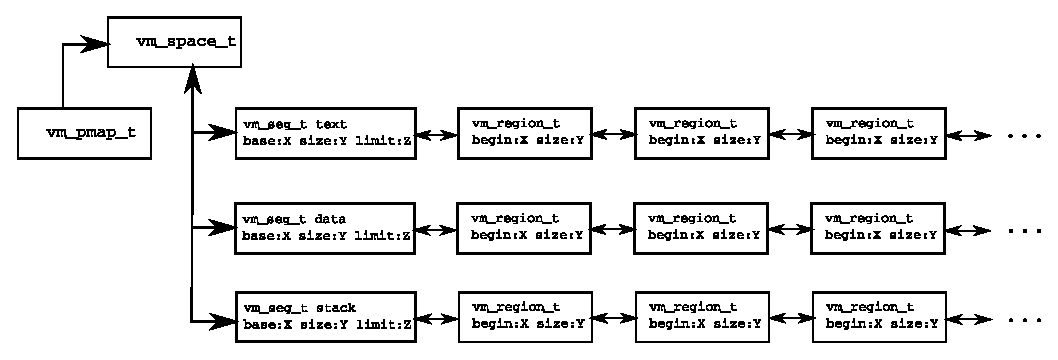
\includegraphics{work/vm_space}
\caption{Techniczne uj�cie przestrzeni adresowej.}
\label{vm:space}
\end{figure}

\subsection{Sterta j�dra.}

\cite{bonwick}

% Impala Operating System
%
% Copyright (C) 2009 University of Wroclaw. Department of Computer Science
%    http://www.ii.uni.wroc.pl/
% Copyright (C) 2009 Mateusz Kocielski, Artur Koninski, Pawel Wieczorek
%    http://trzask.codepainters.com/impala/trac/
% All rights reserved.
%
% Redistribution and use in source and binary forms, with or without
% modification, are permitted provided that the following conditions
% are met:
% 1. Redistributions of source code must retain the above copyright
%  notice, this list of conditions and the following disclaimer.
% 2. Redistributions in binary form must reproduce the above copyright
%  notice, this list of conditions and the following disclaimer in the
%  documentation and/or other materials provided with the distribution.
%
% THIS SOFTWARE IS PROVIDED BY AUTHOR AND CONTRIBUTORS ``AS IS'' AND
% ANY EXPRESS OR IMPLIED WARRANTIES, INCLUDING, BUT NOT LIMITED TO, THE
% IMPLIED WARRANTIES OF MERCHANTABILITY AND FITNESS FOR A PARTICULAR PURPOSE
% ARE DISCLAIMED.  IN NO EVENT SHALL AUTHOR OR CONTRIBUTORS BE LIABLE
% FOR ANY DIRECT, INDIRECT, INCIDENTAL, SPECIAL, EXEMPLARY, OR CONSEQUENTIAL
% DAMAGES (INCLUDING, BUT NOT LIMITED TO, PROCUREMENT OF SUBSTITUTE GOODS
% OR SERVICES; LOSS OF USE, DATA, OR PROFITS; OR BUSINESS INTERRUPTION)
% HOWEVER CAUSED AND ON ANY THEORY OF LIABILITY, WHETHER IN CONTRACT, STRICT
% LIABILITY, OR TORT (INCLUDING NEGLIGENCE OR OTHERWISE) ARISING IN ANY WAY
% OUT OF THE USE OF THIS SOFTWARE, EVEN IF ADVISED OF THE POSSIBILITY OF
% SUCH DAMAGE.
%
% $Id$

\section{Sterowniki urz�dze�.}
\label{DEV}

Sterowniki urz�dze� w~systemach UNIXowych s� widoczne jako pliki. W naszym
systemie zarz�dzaniem takimi plikami zajmuje si� specjalny system plik�w
\texttt{devfs}, zamontowany w~katalogu \texttt{/dev}. Sterowniki urz�dze�
dziel� si� na~trzy kategorie:

\begin{itemize}
 \item urz�dzenia blokowe - sterowniki obs�uguj�ce takie
urz�dzenia jak
stacje dyskietek, dyski twarde itp.
 \item urz�dzenia znakowe - sterowniki obs�uguj�ce
urz�dzenie, widziane jako strumie� bajt�w.
 \item terminale - specjalny rodzaj urz�dze� znakowych.
\end{itemize}

Ka�dy sterownik dostarcza systemowi tak zwan� desk� rozdzielcz�
(\texttt{devsw\_t} - \emph{device switch}), kt�ra zawiera implementacj�
procedur obs�ugi pliku urz�dzenia. Deska rozdz. zawiera nast�puj�ce pola:
\begin{itemize}
 \item \texttt{d\_open} -
obs�uga otwarcie pliku urz�dzenia.

 \item \texttt{d\_close} -
obs�uga zamkni�cia pliku urz�dzenia.

 \item \texttt{d\_ioctl} -
bs�uga polece� kontrolnych dla~sterownika.

 \item \texttt{d\_write} -
obs�uga zlecenia wyj�cie ze strumienia znakowego. mo�e blokowa� klienta
na~czas wykonywania operacji.

 \item \texttt{d\_read} -
obs�uga zlecenia wej�cie ze strumienia znakowego, mo�e blokowa� klienta
na~czas wykonywania operacji.

 \item \texttt{d\_strategy} -
obs�uga zlece� operacji wej�cia-wyj�cia na~urz�dzeniach blokowych, dzia�a
asynchronicznie, tzn nie blokuje klienta na~czas wykonywania operacji.

 \item \texttt{type} -
informacja o kategorii, do jakiej urz�dzenie nale�y
\begin{itemize}
 \item \texttt{DEV\_BDEV} - dla urz�dze� blokowych.
 \item \texttt{DEV\_CDEV} - dla urz�dze� znakowych.
 \item \texttt{DEV\_TTY} - dla terminali.
\end{itemize}
\end{itemize}

Podzia� na urz�dzenia znakowego i~blokowe oraz rozr�nienie procedur
obsluguj�cych zlecenia wej�cia-wyj�cia jest koniecznie ze wzgl�du na~wydajno��
oraz obs�ug� tych urz�dze�. Na~urz�dzeniach znakowych u�ytkownik mo�e
wykonywa� te same operacje jak na plikach, poniewa� pliki s� r�wnie� widziane
jako strumienie znakowe. Dozwolone s� takie operacje jak przeczytanie jednego
bajtu, dw�ch kilobajt�w czy pi�ciu megabajt�w.

Urz�dzenia blokowe jak dyski twarde cechuje inna metod� dost�pu, fizycznie
s� one podzielone na bloki danych (sektory). St�d wszelkie transfery danych
mi�dzy pami�ci� RAM a~urz�dzeniem nie s� tak elastyczne pod~wzgl�dem wielko�ci
jak strumienie znak�w.

Z~powodu tych r�zni� jednolita obs�uga wej�cia-wyj�cia dla~tych dw�ch rodzaj�w
urz�dze� musia�aby emulowa� urz�dzenia blokowe jako znakowe, co nie by�oby
wydajne. Dzi�ki wyodr�bnienie oddzielnej procedury sterownik zawsze dostaje
zlecenia, kt�rych d�ugo�� jest wielokrotno�ci� d�ugo�ci sektoru oraz mo�e sam
zadecydowa� w~jakiej kolejno�ci najlepiej je wykona� (co t�umaczy nazw�
procedury - \emph{strategia}). Mo�liwy jest r�wnie� dost�p strumieniowy
do~takich
urz�dze�, jest on emulowany za~pomoc� procedury \texttt{physio}, kt�ra
wykorzystuje \texttt{d\_strategy}. Nale�y zwr�ci� uwag�, �e jest to~jedynie
dodatkowa metoda dost�pu, przydatna zwykle programom chc�cym bezpo�rednio
modyfikowa� dane na~urz�dzeniu lub ingerowa� w~zapisany tam system plik�w
(jak np programy sorawdzaj�ce powierzchni� dysku czy sp�jno�c systemu plik�w).
Zagadnienie wej�cja-wyj�cia urz�dze� blokowych s� om�wione w~rozdziale
\ref{BIO}.

Operacje wej�cia-wyj�cia na~terminalach dzia�aj� na~tej samej zasadzie
co urz�dze� blokowych, z~t� r�ni� �e te~operacje przechodz� dodatkow�
warstw� zwan� re�imem linii. Te zagadnienia s� szerzej om�wione w~rozdziale
TTY.

W kodzie systemu wi�kszo��, poza specjalnymi, sterownik�w jest wydzielona
do~oddzielnej biblioteki \texttt{libdev.a} (lokalizacja: \texttt{sys/dev/}).
System operacyjny nie zna bezpo�rednio wszystkich
zaimplementowanych w~niej sterownik�w, pobiera natomiast
tablic� \texttt{devtab} zawieraj�c� procedury inicjuj�ce sterowniki.
Specjalnymi sterownikami nie wydzielonymi do~wymienionej biblioteki s�
wirtualne terminale emulowane przez konsol�, kt�ra jest cz�ci� j�dra.

System z~plikami urz�dze� wi��e deskryptor urz�dzenia {\texttt{devd\_t}},
kt�ry zawiera w~sobie takie informacje jak nazwa urz�dzenia, wska�nik
na~prywatne dane sterownika oraz jego desk� rozdzielcz�. Jeden sterownik mo�e
stworzy� wiele deskryptor�w urz�dze�, w zale�no�ci od~tego ile wykryje urz�dze�
kt�re mo�e obs�ugiwa�. Przyk�adowo, zaimplementowany kontroler stacji dyskietek,
je�eli wykryje dwie stacje dyskietek w~komputrze, to tworzy odpowiednio dwa
pliki urz�dze�: \texttt{/dev/fd0} dla stacji \texttt{A:} oraz \texttt{/dev/fd1}
dla stacji \texttt{B:}. System tak� stacj� dyskietek widzi jako dwa r�ne
deskryptory, kt�re wsp�ldziela ze sob� desk� rozdzielcz�.

Nie wszystkie urz�dzenia w~sprz�cie komputerowym s� obs�ugiwane za~pomoc�
tego modelu sterownik�w. Sterowniki niekt�rych urz�dze� mog� by� programowane,
jako modu�y dostarczaj�ce pewn� funkcjonalno��, ni� jako og�lnie dost�pne
pliki urz�dze�. Ta uwaga dotyczy niskopoziomowych urz�dze�, kt�re s�
wykorzystywane przez j�dro do dostarczania pewnych us�ug lub do~implementacji
innych sterownik�w. Udost�pnienie ich jako pliki widziane dla u�ytkownika
nie wnosi�oby �andych korzy�ci, a doda�o trudno�ci implementacyjnych.
Na przyk�ad, sterownik szyny ISA udost�pnia zbi�r procedur
\texttt{bus\_isa\_dma\_} wykorzystywanych w~ sterowniku kontrolera stacji
dyskietek. Sterownik zegara systemowgo instaluje podprogram przerwania,
kt�ry przy ka�dym tykni�ciu uruchamia og�ln� obs�ug� zegara w~systemie.
Obs�uga przerwa� sprz�towych jest om�wiona w~rozdziale \ref{INT}.


\subsection{Szyna ISA.}

Sterownik szyny ISA jest dostarczany przez obs�ug� architektury sprz�tu,
jest on potrzeny w~naszym systemie poniewa� kontroler stacji dyskietek
znajduje si� na~niej. Zadaniem sterownika jest dostarczy� procedury
obs�uguj�ce transfery DMA.

Za obs�ug� transfer�w DMA w komputerach domowych s� odpowiedzialne dwa
kontrolery Intel 8237A. Ka�dy z~nich obs�uguje cztery kana�y, s�u��ce
do wykonywania transfer�w. Ka�de urz�dzenia ma przypisany sw�j kana�, a
przed rozpocz�ciem transferu nale�y go odpowiednio zaprogramowa�.

Deskryptor kana�u musi zosta� przydzielony
za~pomoc� procedury \texttt{bus\_isa\_dma\_alloc}, a programowanie kana��w
odbywa si� przez \texttt{bus\_isa\_dma\_prepare}.
Poniewa� te kontrolery s� star� technologi� to obs�uguj� jedynie transfery
do~fragment�w pami�ci RAM kt�rych adres mi�sci si� w~24 bitach.
Tak� pami�� nie zawsze mo�na przydzieli�, w~szczeg�lno�ci po~d�u�szej pracy
systemu, ten probelm jest rozwi�zany przez przydzielanie sta�ych bufor�w
kana�om przy starcie systemu w~adresach poni�ej 1MB
(zobacz rysunek \ref{vm:mmap}). Po wykonaniu transferu nale�y wykona� procedur�
\texttt{bus\_isa\_dma\_finish}.

Para procedur \texttt{\_prepare} i \texttt{\_finish} kopiuj� odpowiednio
dane pomi�dzy sta�ym buforem kana�u, a~buforem danym przez klienta.

\subsection{Sterownik stacji dyskietek.}

Om�wienie sterownika stacji dyskieteke wymaga uprzedzenia kilku wiadomo�ci
z~rozdzia�u \ref{BIO}.


\subsection{Sztuczne urz�dzenia.}


% Impala Operating System
%
% Copyright (C) 2009 University of Wroclaw. Department of Computer Science
%    http://www.ii.uni.wroc.pl/
% Copyright (C) 2009 Mateusz Kocielski, Artur Koninski, Pawel Wieczorek
%    http://bitbucket.org/wieczyk/impala/
% All rights reserved.
%
% Redistribution and use in source and binary forms, with or without
% modification, are permitted provided that the following conditions
% are met:
% 1. Redistributions of source code must retain the above copyright
%  notice, this list of conditions and the following disclaimer.
% 2. Redistributions in binary form must reproduce the above copyright
%  notice, this list of conditions and the following disclaimer in the
%  documentation and/or other materials provided with the distribution.
%
% THIS SOFTWARE IS PROVIDED BY AUTHOR AND CONTRIBUTORS ``AS IS'' AND
% ANY EXPRESS OR IMPLIED WARRANTIES, INCLUDING, BUT NOT LIMITED TO, THE
% IMPLIED WARRANTIES OF MERCHANTABILITY AND FITNESS FOR A PARTICULAR PURPOSE
% ARE DISCLAIMED.  IN NO EVENT SHALL AUTHOR OR CONTRIBUTORS BE LIABLE
% FOR ANY DIRECT, INDIRECT, INCIDENTAL, SPECIAL, EXEMPLARY, OR CONSEQUENTIAL
% DAMAGES (INCLUDING, BUT NOT LIMITED TO, PROCUREMENT OF SUBSTITUTE GOODS
% OR SERVICES; LOSS OF USE, DATA, OR PROFITS; OR BUSINESS INTERRUPTION)
% HOWEVER CAUSED AND ON ANY THEORY OF LIABILITY, WHETHER IN CONTRACT, STRICT
% LIABILITY, OR TORT (INCLUDING NEGLIGENCE OR OTHERWISE) ARISING IN ANY WAY
% OUT OF THE USE OF THIS SOFTWARE, EVEN IF ADVISED OF THE POSSIBILITY OF
% SUCH DAMAGE.
%
% $Id$

\section{Przerwania.} \label{INT}

Przerwaniem (\emph{interrupt}) jest wyw�aszczenie pracy procesora
przez zdarzenie, kt�re powoduje wykonanie kodu jego obs�ugi.
Przerwania mog� by� generowane przez:
\begin{itemize}
 \item sprz�t komputerowy - nazywamy je wtedy przerwaniami sprz�towymi
 \item kod programu - nazywamy je wtedy przerwaniami programowymi
 \item procesor - nazywamy je wtedy pu�apkami lub wyj�tkami procesora
\end{itemize}

Obs�ug� przerwa� opisuje tablica deskryptor�w dostarczona procesorowi
na~pocz�tku inicjalizacji systemu. W niej s� zapisane takie informacje
jak adres podprogramu obs�ugi oraz poziom uprzywilejowania pracy procesora.
Po zako�czeniu obs�ugi przerwania procesor wraca do~wykonywania wyw�aszczonego
zadania.

Przerwanie mo�e nadej�� w~ka�dym momencie pracy, pomi�dzy dowolnymi
instrukcjami procesora. W systemie z~podzia�em czasu stwarza
to~ryzyko uszkodzenia struktur danych, kt�re s� jednocze�nie modyfikowane
przez wyw�aszczony program oraz obs�ug� danego przerwania. Np. sterownik
stacji dyskietek obs�uguj�c przerwanie mo�e pobra� zlecenie wej�cia-wyj�cia
z~kolejki, kt�ra w�a�nie by�a modyfikowana przez wyw�aszczony program, chc�cy
zakolejkowa� kolejne zlecenie.

Problem jest rozwi�zywany przez wprowadzenia poziom�w uprzywilejowania dla
przerwa�. Przerwania z~ni�szym priorytetem ni� obecny s� odwlekane.
Do zwi�kszania priorytetu s�u�� procedury \texttt{splXXX}, gdzie \texttt{XXX}
jest nazw� poziomu. Zwracaj� one obecny poziom uprzywilejowania.
Procedury nigdy nie zmniejszaj� poziomu uprzywilejowania, co zapobiega
sytuacjom gdzie priorytet zostanie po cichu zmniejszony przez jedn�
z~wykorzystanych procedur w~kodzie maj�cym dzia�a� z wi�kszym.
Priorytet jest przywracany za~pomoc� procedury \texttt{splx}.

Przerwania sprz�towe s� obs�ugiwane przez chipset Intel 8259A\footnote{
Tak naprawd� ten chipset nie jest ju� produkowany, jest obecnie emulowany
przez mostek na p�ycie g��wnej. W nowoczesnych procesorach jest zast�piony
nowym kontrolerem wbudowanym w~procesor.}, za pomoc� niego jest r�wnie�
wykonane manipulowanie poziomami uprzywilejowania i~odwlekania
obs�ugi przerwa�.

Obecnie wyszczeg�lnionymi poziomami uprzywilejowania s�:
\begin{itemize}
 \item \texttt{TTY} - poziom odwleka wszystkie przerwania zwi�zane z~obs�ug�
    terminali, klawiatur.

 \item \texttt{BIO} - poziom odwleka wszystkie przerwania zwi�zane z~obs�ug�
    urz�dze� blokowych.

 \item \texttt{SOFTCLOCK} - poziom odwleka wszystkie przerwania zwi�zane
    z obs�ug� czasomierzy, w~tym zegar systemowy.

 \item \texttt{HIGH} - poziom odwleka wszystkie przerwania w systemie.
\end{itemize}

Manipuluj�c poziomem uprzywilejowania nale�y zwr�ci� szczeg�ln� uwag� na~to,
�e mo�e to~op�nia� obs�ug� urz�dze� przez sterowniki, co mo�e wp�yn��
na~wydajno�� systemu.

Poziom uprzywilejowania mo�na interpretowa� r�wnie� jako element tworzenia
sekcji krytycznych blokuj�cych sterowniki lub zegar systemowy uruchamiaj�cy
program planisty.

Nieuwa�ne mieszanie zmian poziomu uprzywilejowania
z~mechanizmami synchronizacji na~w�tkach mo�e spowodowa� zakleszczenie ca�ego
systemu, poniewa� mechanizmy synchronizacji w�tk�w b�d� czeka� a� inny proces
opu�ci sekcj� krytyczn�, a zmiana poziomu uprzywilejowania wy��czy program
planisty, kt�ry odpowiada za~zmian� aktualnie wykonywanego w�tku.

Sterowniki urz�dze� mog� instalowa� swoje podprogramy obs�ugi za~pomoc�
procedury \texttt{irq\_install\_handler}, przypisuj�c od~razu odpowiedni
poziom uprzywilejowania.

Przerwania b�d�ce wyj�tkami procesora s� przez niego~rzucane w~szczeg�lnych
przypadkach jak nieprawid�owy dost�p do~pami�ci czy wykonanie nieprawid�owej
instrukcji. System Impala zostaje zatrzymany przy ka�dej pu�apce procesora,
opr�cz pu�apki zwi�zanej z~nieodpowiednim dost�pem pami�ci. W takim wypadku,
w zale�no�ci od tego kto wykona� nieprawid�owy dost�p s� podejmowane r�ne
akcje. Je�eli wykona� go proces u�ytkownika to~jest do~niego dostarczany
sygna� \texttt{SIGSEGV}, je�eli j�dro to system jest zatrzymywany.

Przerwania programowe s� wykorzystywane do~komunikacji u�ytkownika z~systemem,
mechanizm jest om�wiony szerzej w~\ref{SYSCALL}.


% Impala Operating System
%
% Copyright (C) 2009 University of Wroclaw. Department of Computer Science
%    http://www.ii.uni.wroc.pl/
% Copyright (C) 2009 Mateusz Kocielski, Artur Koninski, Pawel Wieczorek
%    http://trzask.codepainters.com/impala/trac/
% All rights reserved.
%
% Redistribution and use in source and binary forms, with or without
% modification, are permitted provided that the following conditions
% are met:
% 1. Redistributions of source code must retain the above copyright
%  notice, this list of conditions and the following disclaimer.
% 2. Redistributions in binary form must reproduce the above copyright
%  notice, this list of conditions and the following disclaimer in the
%  documentation and/or other materials provided with the distribution.
%
% THIS SOFTWARE IS PROVIDED BY AUTHOR AND CONTRIBUTORS ``AS IS'' AND
% ANY EXPRESS OR IMPLIED WARRANTIES, INCLUDING, BUT NOT LIMITED TO, THE
% IMPLIED WARRANTIES OF MERCHANTABILITY AND FITNESS FOR A PARTICULAR PURPOSE
% ARE DISCLAIMED.  IN NO EVENT SHALL AUTHOR OR CONTRIBUTORS BE LIABLE
% FOR ANY DIRECT, INDIRECT, INCIDENTAL, SPECIAL, EXEMPLARY, OR CONSEQUENTIAL
% DAMAGES (INCLUDING, BUT NOT LIMITED TO, PROCUREMENT OF SUBSTITUTE GOODS
% OR SERVICES; LOSS OF USE, DATA, OR PROFITS; OR BUSINESS INTERRUPTION)
% HOWEVER CAUSED AND ON ANY THEORY OF LIABILITY, WHETHER IN CONTRACT, STRICT
% LIABILITY, OR TORT (INCLUDING NEGLIGENCE OR OTHERWISE) ARISING IN ANY WAY
% OUT OF THE USE OF THIS SOFTWARE, EVEN IF ADVISED OF THE POSSIBILITY OF
% SUCH DAMAGE.
%
% $Id$

\section{Buforowane wej�cie-wyj�cie (BIO).} \label{bio}

Poniewa� urz�dzenia dyskowe s� o~wiele wolniejsze ni� procesor komputera
to~op�aca si� zapami�tywa� w~pami�ci komputera cz�c danych z~urz�dzenia.
Operacje czytania danych mog� zosta� zrealizowane w~bardzo kr�tkim czasie,
je�eli oka�e si�, �e porz�dane dane z~urz�dzenia s� ju� w~pami�ci.
Za~takie buforowanie operacji na~urz�dzeniach blokowych
(dyskowych) odpowiedzialny jest mechanizm buforowanego wej�cia-wyj�cia.

System pos�uguje si� nag��wkami bufor�w (\texttt{iobuf\_t}).
System przy rozruchu przydziela ustalon� liczb� takich nag��wk�w
(parametr \texttt{iobufs}), a ka�dy z~nich mo�e by� przypisany do~urz�dzenia
oraz numeru bloku(sektoru). Ustalona ilo�c nag��wk�w jest przydzialana przez
system podczas rozruchu (parametr j�dra \texttt{iobufs}) systemu. W celu
przyspieszenia bufory s� trzymane w tablicy haszuj�cej.

\subsection{Tablica haszuj�ca.}

Nag��wki s� nawlekane na~dwie listy, list� wolnych nag��wku je�eli z~danego
buforu nikt nie korzysta oraz na list� tablicy haszuj�cej. Przyk�adowa
tablica jest przedstawiona na rysunku \ref{bio:bufhash}.


\begin{figure}
 \centering
 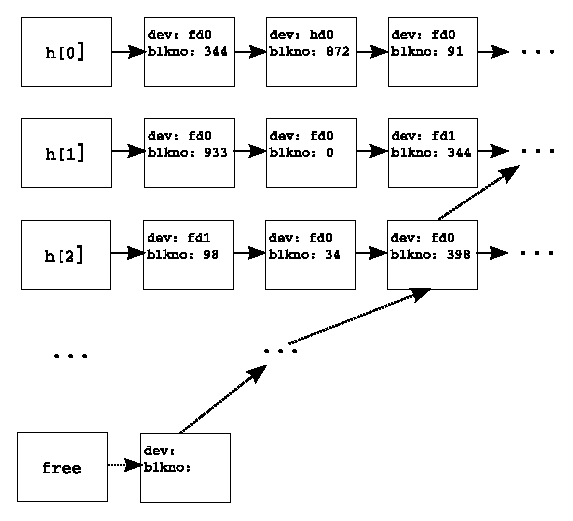
\includegraphics{work/bio_bufhash}
 \caption{Przyk�adowa tablica haszuj�ca. Bloczki z~pierwszej kolumny
 oznaczaja nag��wki list, a z pozosta�ych kolumn nag��wki bufor�w.
 Listy $h[i]$ oznaczaj� listy tablicy haszuj�cej, a \texttt{free} oznacza
 list� wolnych nag��wk�w.
}
 \label{bio:bufhash}
\end{figure}

U�ywana funkcja haszuj�ca wyra�a si� wzorem

\begin{eqnarray*}
 hash(\mbox{\texttt{dev}}, \mbox{{\texttt{blkno}}})
& = &
 h(\mbox{\texttt{adres-deskryptora(dev)}} \times \mbox{{\texttt{blkno}}})\\
 h(k)
& = &
 ((ak + b) \mbox{ mod }p) \mbox{ mod }m
\end{eqnarray*}
 

\subsection{Cykl �ycia nag�owku buforu.}

Poniewa� system pos�uguje si� sta�� ilo�ci� nag��wk�w to~musz� zosta�
ustalone zasady pos�ugiwania si� nimi przez klient�w tego mechanizmu.

Nag��wki s� identyfikowane przez urz�dzenie i~numer bloku, aby pobra� nag��wek
nale�y u�y� procedury \texttt{bio\_getblk}. Procedura sprawdza najpierw, czy
dany sektor z~urz�dzenia nie jest ju� zapami�tany, je�eli nie jest
to~przydziela nag�owek z~listy wolnych oraz organizuje pami�� na bufor.
Zwr�cony nag�owek jest naznaczony jako zawieraj�cy nieprawid�owe dane.

Je�eli nag��wek zawieraj�cy porz�dane sektory znajduje si� w~pami�ci
to~nale�y sprawdzi� czy nie jest w�a�nie u�ywany przez innego klienta. Je�eli
tak to w�tek prosz�cy o~nag��wek jest usypiany, a� do momentu mo�liwo�ci
przydzielania buforu. W przeciwnym wypadku nale�y naznaczy� nag��wek
jako~u�ywany i~go zwr�ci�.

Inn� drog� otrzymania nag��wku urz�dzenia jest procedura \texttt{bio\_read},
kt�ra jest nak�adk� na~procedur� om�wion� wy�ej. Jej zadaniem jest zlecenie
operacji wej�cia-wyj�cia sterownikowi urz�dzenia je�eli zwr�cony nag�owek
jest nieprawid�owy. W tym przypadku r�wnie� blokuje obecny w�tek na~czas
wykonania operacji przez sterownik.

Otrzymany nag��wek nale�y zwr�ci� do mechanizmu za~pomoc� procedury
\texttt{bio\_release} lub \texttt{bio\_write}, gdzie druga, jak wskazuje
nazwa, wysy�a dane z~buforu do~urz�dzenia.

Procedura \texttt{bio\_wait} s�u�y do~oczekiwania zako�czenia operacji
wej�cia-wyj�cia wykorzystuj�cej dany bufor, jest wewn�trznie wykorzystywana
przez \texttt{bio\_read} i \texttt{bio\_write}. Sterowniki urz�dze� pos�uguj�
si� procedurami \texttt{bio\_done} i \texttt{bio\_error} w~celu poinformowania
mechanizmu o zako�czeniu.
% Impala Operating System
%
% Copyright (C) 2009 University of Wroclaw. Department of Computer Science
%    http://www.ii.uni.wroc.pl/
% Copyright (C) 2009 Mateusz Kocielski, Artur Koninski, Pawel Wieczorek
%    http://bitbucket.org/wieczyk/impala/
% All rights reserved.
%
% Redistribution and use in source and binary forms, with or without
% modification, are permitted provided that the following conditions
% are met:
% 1. Redistributions of source code must retain the above copyright
%  notice, this list of conditions and the following disclaimer.
% 2. Redistributions in binary form must reproduce the above copyright
%  notice, this list of conditions and the following disclaimer in the
%  documentation and/or other materials provided with the distribution.
%
% THIS SOFTWARE IS PROVIDED BY AUTHOR AND CONTRIBUTORS ``AS IS'' AND
% ANY EXPRESS OR IMPLIED WARRANTIES, INCLUDING, BUT NOT LIMITED TO, THE
% IMPLIED WARRANTIES OF MERCHANTABILITY AND FITNESS FOR A PARTICULAR PURPOSE
% ARE DISCLAIMED.  IN NO EVENT SHALL AUTHOR OR CONTRIBUTORS BE LIABLE
% FOR ANY DIRECT, INDIRECT, INCIDENTAL, SPECIAL, EXEMPLARY, OR CONSEQUENTIAL
% DAMAGES (INCLUDING, BUT NOT LIMITED TO, PROCUREMENT OF SUBSTITUTE GOODS
% OR SERVICES; LOSS OF USE, DATA, OR PROFITS; OR BUSINESS INTERRUPTION)
% HOWEVER CAUSED AND ON ANY THEORY OF LIABILITY, WHETHER IN CONTRACT, STRICT
% LIABILITY, OR TORT (INCLUDING NEGLIGENCE OR OTHERWISE) ARISING IN ANY WAY
% OUT OF THE USE OF THIS SOFTWARE, EVEN IF ADVISED OF THE POSSIBILITY OF
% SUCH DAMAGE.
%
% $Id: vfs.tex 486 2009-06-25 07:51:47Z wieczyk $

\section{Interfejs terminali.}
\label{TTY}
Programy u�ytkownika wymagaj� od systemu ujednoliconego dost�pu do urz�dze�
umo�liwiaj�cych im komunikacj� z u�ytkownikiem. Urz�dzenia s�u��ce do takiej
komunikacji nazywamy terminalami. Terminale mo�na podzieli� na nast�puj�ce grupy:
\begin{enumerate}
\item Terminal zewn�trzny, komunikuj�cy si� z komputerem poprzez port szeregowy
b�d� modem
\item Terminal zintegrowany z komputerem, komunikacja nast�puje np. poprzez
dzielon� pami��. (Klawiatura, monitor)
\item Terminal sieciowy - komunikacja np. poprzez Ethernet
\end{enumerate}
Wszystkie te urz�dzenia widoczne s� dla u�ytkownika w ujednoliconej formie - jako
urz�dzenia terminalowe. W systemie Impala z terminalami zwi�zana jest struktura
\texttt{tty\_t}. Rejestrowanie nowego urz�dzenia terminalowego w systemie
nast�puje poprzez funkcj� \texttt{tty\_create}. Jako argumenty przyjmuje ona
nazw� nowego urz�dzenia, dowoln� struktur� z prywatnymi danymi urz�dzenia, oraz
wska�nik do funkcji obs�uguj�cej zapis na tym urz�dzeniu. W ten spos�b, system
terminali stanowi nak�adk� na inne urz�dzenia, implementuj�c� ich typowe
funkcjonalno�ci w zunifikowany spos�b.
\subsection{Re�im linii.}
Aby zapewni� zgodno�� program�w Unixowych z oferowanym przez nas interfejsem
terminali, zosta� on zaprojektowany zgodnie ze standardem POSIX dotycz�cym tej
kwestii. Standard reguluje jak ma przebiega� wej�cie, wyj�cie oraz zmiana
ustawie� terminala.
\subsubsection{Zmiana ustawie�.}
Najwa�niejsze ustawienia terminala przechowywane s� w strukturze \texttt{termios}.
Zawiera ona nast�puj�ce pola:

\begin{center}
\begin{tabular}{|l|l|}
\hline
tcflag\_t c\_iflag & Flagi konfiguruj�ce zachowanie wej�cia\\
tcflag\_t c\_oflag & Flagi konfiguruj�ce zachowanie wyj�cia\\
tcflag\_t c\_lflag & Og�lne flagi ustawiaj�ce tryb pracy terminala\\
tcflag\_t c\_cflag & Flagi zwi�zane z obs�ug� po��czenia\\
cc\_t c\_cc[NCCS] & Znaki specjalne \\
\hline
\end{tabular}
\end{center}

Przeznaczenie poszczeg�lnych p�l zostanie przybli�one w kolejnych podrozdzia�ach.
Biblioteka C udost�pnia funkcje do zapisu i odczytu aktualnych ustawie� terminala
- s� to odpowiednio \texttt{tcsetattr} i \texttt{tcgetattr}. Funkcje to zosta�y
zaimplementowane w oparciu o wywo�anie systemowe \texttt{ioctl}.
\subsubsection{Otwieranie terminala, uprawnienia proces�w.}
Terminal otwierany jest jak zwyk�y plik, przy pomocy wywo�ania systemowego
\texttt{open}. Aby umo�liwi� wielu programom jednoczesne korzystanie z jednego
terminala, oraz umo�liwi� kontrol� zada� w pow�okach takich jak \texttt{ash},
wprowadzona zosta�a dodatkowa organizacja proces�w.

Ka�dy proces mo�e posiada� sw�j powi�zany terminal kontroluj�cy. Og�lnie rzecz
bior�c, mo�e on korzysta� tylko z tego terminala.
Procesy zosta�y podzielone na sesje, oraz w ramach sesji na grupy.
Wszystkie procesy w ramach sesji, kt�re maj� ustawiony terminal kontroluj�cy,
maj� ustawiony ten sam terminal. Tak wi�c terminal jest powi�zany z sesj�.
Terminal mo�e by� zwi�zany z tylko jedn� sesj� i vice versa.

W ramach sesji procesy tworz� roz��czne grupy, z kt�rych jedna mo�e by�
wyszczeg�lniona jako grupa proces�w pierwszoplanowych terminala. Procesy z tej
grupy jako jedyne maj� dost�p do wej�cia z terminala. Co do zapisu na terminal,
mo�liwy jest on tak�e spoza grupy proces�w pierwszoplanowych, jednak to wymaga
dodatkowych �rodk�w (w postaci blokowania lub ignorowania sygna�u \texttt{SIGTTOU}).

Sesja oraz grupa proces�w posiadaj� sw�j identyfikator, r�wny identyfikatorowi
procesu, kt�ry jako pierwszy do danego bytu nale�a�.
Proces taki zwany jest odpowiednio liderem sesji i liderem grupy.
Do tworzenia nowej sesji wykorzystuje si� funkcj� \texttt{setsid}.
Terminal kontroluj�cy procesu ustawiany jest automatycznie, w momencie
otwierania go, o ile proces otwieraj�cy nie posiada ju� terminala kontroluj�cego,
jest liderem sesji, oraz terminal ten nie jest jeszcze zwi�zany z �adn� sesj�.
Terminal kontroluj�cy, sesj�, oraz grup� proces dziedziczy po ojcu w wywo�aniu
\texttt{fork}.

Pobieranie i modyfikacja grupy procesu realizowane s� poprzez \texttt{getpgid}
i \texttt{setpgid}. Wyb�r grupy proces�w pierwszoplanowych terminalu nast�puje
poprzez wywo�anie \texttt{ioctl} na deskryptorze pliku terminala, z poleceniem
\texttt{TIOCSPGRP} (zobacz tak�e \texttt{tcsetpgrp} i \texttt{tcgetpgrp}).
\subsubsection{Zapisywanie do terminala.}
% Mo�na wywali� / skr�ci�, w zwi�zku z powielaniem tre�ci ju� opisanych
Programy przekazuj� dane na wyj�cie terminala za pomoc� jednej z funkcji biblioteki C,
zazwyczaj z rodziny \texttt{printf}.
Funkcja \texttt{printf} wywo�uje poprzez przerwanie systemow� funkcj� \texttt{sc\_write}.
Ta z koleji, poprzez vnode zwi�zany z deskryptorem pliku przekazuje bufor z danymi
u�ytkownika do funkcji obs�ugi \texttt{tty\_write} urz�dzenia znakowego zwi�zanego z terminalem.

Zanim b�dzie m�g� nast�pi� faktyczny zapis danych przy pomocy funkcji zarejestrowanej
w procedurze \texttt{tty\_create}, funkcja \texttt{tty\_write} weryfikuje, czy
pisz�cy proces ma do tego prawo, oraz w zale�no�ci od ustawie� wykonuje ko�cowe
przekszta�cenia na danych u�ytkownika. Wykonywane przekszta�cenia uzale�nione s�
od warto�ci \texttt{c\_oflag}. Mo�liwe operacje to miedzy innymi zamiana znak�w
\texttt{CR} (powr�t karetki) na znaki \texttt{NL} (nowej linii) i zamiana znak�w
\texttt{NL} na par� \texttt{CR-NL}.

\subsubsection{Odczyt z terminala.}
Urz�dzenie wej�ciowe otrzymawszy dane, przekazuje je do bufora powi�zanego terminala
poprzez funkcj� \texttt{tty\_input}. U�ytkownik uzyskuje dost�p do tych danych
przy pomocy funkcji bibliotecznych takich jak \texttt{scanf}, korzystaj�cych z wywo�ania
systemowego \texttt{read}. Dane uzyskane w ten spos�b to ci�g znak�w ASCII.

Wyobra�my sobie nast�puj�c� sytuacj�: program pyta u�ytkownika, o podanie imienia,
ten jednak, w po�owie wpisywanego tekstu pope�ni� b��d i skorygowa� go przy u�yciu
klawisza backspace. Program jest zainteresowany jedynie poprawionym wpisem, a nie
ci�giem znak�w zawieraj�cych b��dne dane oraz kod ASCII klawisza backspace.
Jest to na tyle cz�sta sytuacja, �e schemat obs�ugi wej�cia, w kt�rym sterownik
dba o obs�ug� zmian w ramach jednej lini wej�cia zosta� uwzgl�dniony w standardzie
POSIX jako element interfejsu terminali. Oczywi�cie niekt�re programy chc�
zna� kody wszystkich naciskanych klawiszy, bez konieczno�ci czekania na znak
nowej lini, tak wi�c i ta sytuacja musi by� obs�ugiwana. Pierwszy tryb wed�ug
POSIX zwiemy trybem kanoniczym, drugi surowym. Tryb pracy terminala uzale�niony jest od
obecno�ci flagi \texttt{ICANON} w polu \texttt{c\_lflag} struktury opisuj�cej
konfiguracj� terminala.
\subsubsection{Tryb kanoniczny.}
Domy�lnie terminal znajduje si� w trybie kanonicznym.
W trybie tym rozpoznawane s� znaki specjalne, ustalone w polach tabeli
\texttt{c\_cc}. Nale�� do nich EOF, EOL, ERASE, INTR, KILL, QUIT, START, STOP,
SUSP i TIME. Sterownik dokonuje edycji linii w przypadku rozpoznania znaku ERASE
(usuni�cie ostatniego znaku) b�d� KILL (usuni�cie ca�ej lini). Je�eli pole
\texttt{c\_lflag} zawiera flag� \texttt{ISIG}, wyst�pienie znak�w INTR, QUIT
oraz SUSP powoduje wys�anie do grupy proces�w pierwszoplanowych odpowiednio
sygna�u \texttt{SIGINT}, \texttt{SIGQUIT}, \texttt{SIGTSTP}.

Procedura \texttt{read} zwraca wynik, tylko w przypadku gdy
w buforze wej�ciowym terminala istnieje linia zako�czona znakiem NL, EOF b�d� EOL.
Je�eli linia nie jest jeszcze gotowa, proces zasypia w oczekiwaniu na ni�.
Zwr�cony bufor zawiera co najwy�ej jedn� lini� z wej�cia.

W trybie kanonicznym na wej�ciu wykonywane jest wst�pne przetwarzanie,
wed�ug warto�ci \texttt{c\_iflag}. Mo�liwe operacje to m.in. ignorowanie znak�w
\texttt{CR}, zamiana znaku \texttt{CR} na znak \texttt{NL} i na odwr�t.
\subsubsection{Tryb surowy.}
W trybie surowym znaki nie s� dodatkowo przetwarzane. Poprzez ustawienie p�l
\texttt{c\_cc[VMIN]} i \texttt{c\_cc[VTIME]} u�ytkownik mo�e kontrolowa�
minimaln� ilo�� znak�w, jaka zostanie zwr�cona przez \texttt{read}, oraz czas,
jaki procedura ma czeka� na kolejny znak (b�d� ca�o�� wej�cia - przy \texttt{MIN}$=0$).
\subsection{Konsola.}
Jedynym w tej chwili zaimplementowanym w Impali terminalem jest konsola - zestaw
z�o�ony z klawiatury i wy�wietlacza pod��czonego do karty graficznej.
Urz�dzenia te s� widoczne w systemie jako kilka osobnych wirtualnych konsoli,
o plikach \texttt{/dev/ttyvX}, gdzie \texttt{X} jest numerem urz�dzenia.
Prze��czanie pomi�dzy tymi konsolami nast�puje po naci�ni�ciu odpowiedniego
klawisza funkcyjnego \texttt{Fx}.
\subsubsection{Obs�uga klawiatury.}
Niskopoziomowa obs�uga klawiatury przebiega nast�puj�co:
\begin{itemize}
\item Ka�de wci�ni�cie i zwolnienie klawisza powoduje wygenerowanie przerwania
klawiatury.
\item Procedura obs�ugi tego przerwania rozpoznaje rodzaj zdarzenia,
odczytuj�c jego kod - "scancode" - z odpowiedniego portu uk�adu kontrolera
klawiatury (i8042).
\item Na podstawie scancode wyznaczany jest unikalny kod klawisza - "keycode".
\item Na podstawie kodu klawisza, przechowywanych w sterowniku informacji
o naci�ni�tych klawiszach specjalnych takich jak shift, alt i ctrl
oraz "keymapy" odwzorowuj�cej te informacje w znak (ewentualnie ci�g znak�w)
ASCII, wyznaczany jest wynik naci�ni�cia klawisza w postaci, jakiej oczekuje
u�ytkownik.
\item Wynik z poprzedniego kroku przekazywany jest do aktywnej wirtualnej
konsoli oraz powi�zanego z ni� terminala poprzez procedur�
\texttt{vcons\_input\_[char/string]}.
\end{itemize}
\subsubsection{Obs�uga karty graficznej.}
Niskopoziomowa komunikacja z kart� graficzn� w Impali polega na:
\begin{itemize}
\item Pocz�tkowym zainicjalizowaniu karty graficznej, realizowanym poprzez
odpowiedni� sekwencj� zapis�w i odczyt�w z port�w karty. W kroku tym
ustawiany jest m.in. kursor sprz�towy. Poniewa� nie ma mo�liwo�ci wy��czenia
migania kursora sprz�towego, zostaje on ukryty. Kursor widoczny na ekranie jest
emulowany programowo.
\item Bufor ramki karty graficznej jest odwzorowany w pami�� pod adresem fizycznym\\
\texttt{0xb8000}. Jako, �e w Impali niskie adresy s� zarezerwowane na przestrze�
u�ytkownika, ten adres fizyczny jest z koleji odwzorowywany w stercie j�dra.
Wy�wietlenie znaku w pewnym miejscu ekranu polega na
zapisaniu go w odpowiednim miejscu pami�ci. Atrybuty znak�w takie jak ich kolor
dla znaku z kom�rki pami�ci $x$ ustawiane s� w kom�rce $x+1$.
\end{itemize}
\subsection{Emulacja terminala.}
Aby umo�liwi� programom u�ytkownika bardziej zaawansowan� kontrol� nad
zawarto�ci� ekranu, wirtualne konsole udaj�, �e s� fizycznym terminalem.
Konsola w Impali emuluje VT100, popularny terminal stworzony przez
firm� Digital Equipment Corporation. Emulacja ta polega na rozpoznawaniu
sekwencji steruj�cych tego terminala oraz odpowiednim reagowaniu na nie.
Podobnie, wej�cie z klawiatury przedstawiane jest u�ytkownikowi w postaci, jak�
by otrzyma� pracuj�c na terminalu VT100 i korzystaj�c z jego klawiatury.

Dzi�ki takim dzia�aniom progamy maj� mo�liwo�� m.in. ustawia� pozycj� kursora
na ekranie, przewija� ekran, kasowa� jego zawarto��, pobiera� informacje
o po�o�eniu kursora i o wspieranych funkcjonalno�ciach, zmienia� tryb pracy
terminala i atrybuty wypisywanych znak�w.
\begin{table}
\begin{tabular}{|l|l|}
\hline
ESC[2J & Czy�ci ca�y ekran \\
ESC3C & Przesuwa kursor o 3 pozycje w prawo \\
ESC[1;5H & Ustawia kursor w pi�tej kolumnie pierwszego wiersza \\
ESC[5;7;1m & W��cza mruganie, pogrubienie oraz zamienia kolor t�a z kolorem znaku \\
ESC[6n & ��da informacji o aktualnym po�o�eniu kursora \\
\hline
\end{tabular}
\caption{Przyk�adowe sekwencje steruj�ce VT100. ESC oznacza znak \texttt{$\backslash$033}}
\end{table}

%mo�na da� ma�� tabelk� z przyk�adowymi sekwencjami
\subsection{Termcap.}
Jako, �e istnieje wiele terminali, r�ni�cych si� sekwencjami
steruj�cymi, rozmiarem ekranu i innymi szczeg�ami ich dzia�ania, wynik�a
potrzeba udost�pniania procesowi informacji o terminalu na jakim aktualnie
dzia�a. Identyfikator tego terminala przechowywany jest w zmiennej �rodowiskowej
\texttt{TERM}. Dost�p do informacji o konkretnych sekwencjach steruj�cych
mo�liwy jest poprzez nast�puj�ce funkcje biblioteki C: \texttt{tgetstr},
\texttt{tgetnum}, \texttt{tgetflag}. Zanim jednak b�dziemy mogli skorzysta�
z tych funkcji, konieczne jest za�adowanie informacje o wybranym terminalu
za pomoc� funkcji \texttt{tgetent}. Informacje uzyskane z wymienionych funkcji
mog� s�u�y� jako wej�cie do procedury \texttt{tgoto}, wype�niaj�cej sekwencj�
steruj�c� o wymagane argumenty, oraz procedury \texttt{tputs} wysy�aj�cej
sekwencj� do terminala.

Baza danych dla termcap typowo przechowywana w pliku, jest u nas dost�pna
jako warto�� zmiennej �rodowiskowej \texttt{TERMCAP}.

% Impala Operating System
%
% Copyright (C) 2009 University of Wroclaw. Department of Computer Science
%    http://www.ii.uni.wroc.pl/
% Copyright (C) 2009 Mateusz Kocielski, Artur Koninski, Pawel Wieczorek
%    http://trzask.codepainters.com/impala/trac/
% All rights reserved.
%
% Redistribution and use in source and binary forms, with or without
% modification, are permitted provided that the following conditions
% are met:
% 1. Redistributions of source code must retain the above copyright
%  notice, this list of conditions and the following disclaimer.
% 2. Redistributions in binary form must reproduce the above copyright
%  notice, this list of conditions and the following disclaimer in the
%  documentation and/or other materials provided with the distribution.
%
% THIS SOFTWARE IS PROVIDED BY AUTHOR AND CONTRIBUTORS ``AS IS'' AND
% ANY EXPRESS OR IMPLIED WARRANTIES, INCLUDING, BUT NOT LIMITED TO, THE
% IMPLIED WARRANTIES OF MERCHANTABILITY AND FITNESS FOR A PARTICULAR PURPOSE
% ARE DISCLAIMED.  IN NO EVENT SHALL AUTHOR OR CONTRIBUTORS BE LIABLE
% FOR ANY DIRECT, INDIRECT, INCIDENTAL, SPECIAL, EXEMPLARY, OR CONSEQUENTIAL
% DAMAGES (INCLUDING, BUT NOT LIMITED TO, PROCUREMENT OF SUBSTITUTE GOODS
% OR SERVICES; LOSS OF USE, DATA, OR PROFITS; OR BUSINESS INTERRUPTION)
% HOWEVER CAUSED AND ON ANY THEORY OF LIABILITY, WHETHER IN CONTRACT, STRICT
% LIABILITY, OR TORT (INCLUDING NEGLIGENCE OR OTHERWISE) ARISING IN ANY WAY
% OUT OF THE USE OF THIS SOFTWARE, EVEN IF ADVISED OF THE POSSIBILITY OF
% SUCH DAMAGE.
%
% $Id$

\section{Wirtualny system plik�w (VFS).}
\label{VFS}
% no wi�c najpierw przyda� by si� jaki� wst�p, info o tym, czym s� pliki, jak
% wygl�da ich obs�uga od strony u�ytkownika
% potem o 
\subsection{Pliki od strony u�ytkownika.}
Interfejs plik�w jest jednym z najwa�niejszych interfejs�w jakie programy
maj� do dyspozycji. W systemach UNIX'owych pliki reprezentuj� ca�� gam� byt�w:
\begin{itemize}
\item Pliki w standardowym rozumieniu, jako pewnej d�ugo�ci ci�g bajt�w. Jest
to rodzaj pliku, z jakim u�ytkownik najcz�ciej ma kontakt, korzystaj�c
z~sytem�w plik�w takich FAT, NTFS, UFS, ext3 itd.
\item Urz�dzenia - zar�wno fizycznie istniej�ce w komputerze, jak i wirtualne.
\item Potoki FIFO
\item Pliki jako wirtualne byty s�u��ce do przekazywania r�nych informacji 
z~j�dra systemu.
\end{itemize}
Niezale�nie od tego, co kryje si� pod plikiem, od strony u�ytkownika posiada
on jednolity interfejs. Najwa�niejszymi funkcjami wchodz�cymi w jego sk�ad s�:
\texttt{open}, \texttt{close}, \texttt{read}, \texttt{write}, \texttt{ioctl}
\texttt{fcntl}, \texttt{fseek} i \texttt{fstat}. Otwarty plik w programie jest
identyfikowany przy pomocy deskryptora pliku - zazwyczaj ma�ej liczby nieujemnej.
J�dro systemu posiada zwi�zan� z ka�dym procesem tabel�, s�u��c� do t�umaczenia
deskryptora pliku na struktur� \texttt{file\_t}. Wiele deskryptor�w plik�w mo�e
wskazywa� na t� sam� struktur�. Oto, jak wygl�da \texttt{file\_t}:

\begin{center}
\begin{tabular}{|ll|l|}
\hline
vnode\_t   & *f\_vnode & Wska�nik na v-w�ze� zwi�zany z plikiem\\
off\_t     &  f\_offset & Aktualna pozycja kursora w pliku\\
int       &  f\_refcnt & Licznik referencji dla tej struktury\\
int       &  f\_flags & Flagi, pocz�tkowo ustawione przez open\\
\hline
\end{tabular}
\end{center}
 
Tak wi�c wszystkie deskryptory wskazuj�ce na ten sam plik dziel� informacje
takie jak aktualna pozycja kursora oraz flagi pliku.

\subsection{Pliki od strony j�dra.}

Wa�nym zadaniem j�dra systemu operacyjnego jest stworzenie takich warunk�w,
w kt�rych pliki pochodz�ce z r�nych system�w plik�w mog� by� obs�ugiwane
przez pojedynczy, uniwersalny interfejs. Takie w�a�nie zadanie spe�nia
VFS - wirtualny system plik�w. Zar�wno poj�cie pliku jak i systemu plik�w
zosta�o uj�te w ramy �ci�le zdefiniowanych struktur j�dra, ukrywaj�cych
prawdziw� implementacj� powi�zanych z nimi operacji. Pliki s� reprezentowane
przez struktur� \texttt{vnode\_t}, natomiast systemy plik�w poprzez 
\texttt{vfs\_t}. Implementacja zawarta w Impali bazowana by�a na tej z SVR4.
\subsubsection{V-w�z�y}
Aby m�c zrozumie� funkcjonowanie wirtualnego systemu plik�w, wa�n� jest
znajomo�� struktury, do kt�rej odnosi si� wi�kszo�� operacji.
Oto jak wygl�da v-w�ze�:

\begin{center}
\begin{tabular}{|l l| l|}
\hline
int            &~v\_type        & typ v-w�z�a\\
int            &~v\_flags       & flagi v-w�z�a\\
int            &~v\_refcnt      & licznik referencji\\
vfs\_t         &*v\_vfs\_mounted\_here & system plik�w tutaj zamontowany\\
vfs\_t         &*v\_vfs         & system plik�w tego vnode\\
vnode\_ops\_t  &*v\_ops         & wska�nik do \texttt{vnode\_ops} z tego fs\\
devd\_t        &*v\_dev         & urz�dzenie, je�li to v-w�ze� urz�dzenia\\
void           &*v\_private     & prywatne dane systemu plik�w, np. i-w�ze�\\
mutex\_t       &~v\_mtx         & blokada do synchronizacji\\
\hline
\end{tabular}
\end{center}

Impala posiada nast�puj�ce typy v-w�z��w:
\begin{center}
\begin{tabular}{lcl}
VNODE\_TYPE\_REG & - &zwyk�y plik \\
VNODE\_TYPE\_DIR & - &plik reprezentuj�cy katalog \\
VNODE\_TYPE\_DEV & - &plik reprezentuj�cy urz�dzenie \\
VNODE\_TYPE\_LNK & - &plik b�d�cy dowi�zaniem symbolicznym \\
VNODE\_TYPE\_FIF & - &plik reprezentuj�cy potok \\
\end{tabular}
\end{center}

Operacje mo�liwe do wykonania na v-w�le ukryte s� w strukturze
\texttt{vnode\_ops\_t} dostarczanej dla ka�dego v-w�z�a przez zwi�zany z nim
system plik�w. Struktura ta zawiera wska�niki do funkcji wykonuj�cych wszystkie
przewidzane przez nas operacje, jakie s� mo�liwe do wykonania na pliku.
Szczeg�owo zosta�a ona przedstawiona w tabeli \ref{vnodeops}.

Dla wygody korzystania z v-w�z��w dla ka�dej z operacji wprowadzono
odpowiednie makro \texttt{VOP\_XXX(v, ...)} wykonuj�ce operacj� \texttt{XXX}
na v-w�le \texttt{v}.
Dla dalszego u�atwienia pracy z v-w�z�ami, wprowadzono nast�puj�ce og�lne
procedury:
\begin{itemize}
\item \texttt{vnode\_opendev} - otwiera vnode urz�dzenia o podanej nazwie
\item \texttt{vnode\_rdwr}, \texttt{vnode\_urdwr} - wykonuj� operacje odczytu
i zapisu do danego v-w�z�a
\item \texttt{vnode\_stat} - pobiera r�ne informacje o pliku
\item \texttt{vnode\_isatty} - sprawdza czy v-w�ze� zwi�zany jest z urz�dzeniem
terminalowym
\item \texttt{vnode\_access\_ok} - weryfikuje uprawnienia danego procesu do
dost�pu do pliku z zamiarem wykonania podanych operacji
\item \texttt{vnode\_alloc} - przydziela now�, pust� struktur� v-w�z�a
\item \texttt{vrele} - zwalnia dan� referencj� do v-w�z�a
\item \texttt{vref} - tworzy now� referencj� do v-w�z�a
\end{itemize}
W kwestii zliczania referencji, przyj�ta przez nas strategia zak�ada, �e
ka�da funkcja zwracaj�ca w wyniku v-w�ze�, musi zwr�ci� go ze zwi�kszon� ju�
liczb� referencji (tj. wykonanym \texttt{vref}). Dzi�ki temu, eliminujemy
jedn� z mo�liwych sytuacji wy�cigu. Procedura wywo�uj�ca staje si� w ten spos�b
w�a�cicielem zwr�conego wska�nika do v-w�z�a. Je�eli nie b�dzie ju� wi�cej z
niego korzysta�a, musi wykona� na nim \texttt{vrele}.

Kolejnym ustaleniem, jest to, �e funkcja, kt�ra dosta�a v-w�ze� jako argument,
mo�e bez przeszk�d z niego korzysta�, o ile nie zachowuje tego wska�nika na p�niej.
Ka�de klonowanie wska�nika wymaga wywo�ania funkcji \texttt{vref}.
Wyra�nie oznaczone funkcje mog� jednak przejmowa� prawo w�asno�ci do referencji
od strony wywo�uj�cej. Jest to wykorzystywane dla wygody, w sytuacjach, gdy po
wykonaniu procedury dalszy dost�p do obiektu nie jest zazwyczaj potrzebny.

Podobna strategia zosta�a zastosowana w odniesieniu do struktury \texttt{file\_t}.
Odpowiednie funkcje maj� nazwy \texttt{frele} i \texttt{fref}.

W przypadku zwalniania ostatniej referencji do v-w�z�a, wykonywana jest na nim
operacja \texttt{VOP\_INACTIVE}, maj�ca na celu poinformowanie i-w�z�a (zale�nej
od sytemu plik�w cz�ci v-w�z�a) o tej sytuacji. Umo�liwi to wykonanie ko�cowych
czynno�ci, takich jak zwolnienie i-w�z�a.
\begin{table}
\begin{tabular}{|l l|p{9cm}|}
\hline
vnode\_open\_t      &*vop\_open&Otwieranie pliku \\
vnode\_create\_t    &*vop\_create&Tworzenie nowego pliku \\
vnode\_close\_t     &*vop\_close&Zamykanie pliku \\
vnode\_read\_t      &*vop\_read&Odczytywanie z pliku \\
vnode\_write\_t     &*vop\_write&Zapisywanie do pliku \\
vnode\_ioctl\_t     &*vop\_ioctl&Wykonywanie dodatkowych operacji \\
vnode\_seek\_t      &*vop\_seek&Sprawdzanie, czy dana pozycja jest prawid�owa\\
vnode\_truncate\_t  &*vop\_truncate&Zmiana rozmiaru pliku\\
vnode\_getattr\_t   &*vop\_getattr&Pobieranie r�nych atrybut�w pliku\\
vnode\_setattr\_t   &*vop\_setattr&Ustawianie atrybut�w pliku\\
vnode\_lookup\_t    &*vop\_lookup&Poszukiwanie v-w�z�a o podanej nazwie, pocz�wszy
    od danego v-w�z�a katalogu\\
vnode\_mkdir\_t     &*vop\_mkdir&Tworzenie nowego katalogu\\
vnode\_getdents\_t  &*vop\_getdents&Pobieranie zawarto�ci katalogu\\
vnode\_readlink\_t  &*vop\_readlink&Odczytywanie nazwy pliku na kt�ry wskazuje
    dowi�zanie symboliczne\\
vnode\_symlink\_t   &*vop\_symlink&Tworzenie dowi�zania symbolicznego\\
vnode\_access\_t    &*vop\_access&Sprawdzanie praw dost�pu do pliku\\
vnode\_sync\_t      &*vop\_sync&Synchronizowanie stanu pliku w pami�ci ze stanem
    na trwa�ym no�niku\\
vnode\_inactive\_t  &*vop\_inactive&Informowanie pliku, �e ostatnia referencja
do tego v-w�z�a jest w�a�nie usuwana\\
vnode\_lock\_t      &*vop\_lock&Blokowanie pliku\\
vnode\_unlock\_t    &*vop\_unlock&Odblokowywanie pliku\\
vnode\_rmdir\_t     &*vop\_rmdir&Usuwanie katalogu\\
vnode\_link\_t      &*vop\_link&Podwi�zywanie istniej�cego pliku pod now� nazw�\\
vnode\_unlink\_t    &*vop\_unlink&Usuwanie wpisu z katalogu\\
\hline
\end{tabular}
\caption{Struktura v-w�z�a - \texttt{vnode\_t}}
\label{vnodeops}
\end{table}
\subsection{Systemy plik�w}
Struktura reprezentuj�ca zamontowane systemy plik�w jest analogiczna do
struktury v-w�z�a, jednak�e zwi�zane z ni� operacje s� mniej liczne:
\begin{center}
\begin{tabular}{|l l| l|}
\hline
vfs\_ops\_t    &*vfs\_ops &   definicje operacji zwi�zanych z tym systemem plik�w\\
vnode\_t      &*vfs\_mpoint &  v-w�ze� kt�ry przykryli�my montuj�c ten s. plik�w\\
devd\_t       &*vfs\_mdev &    urz�dzenie, u�ywane przez ten s. plik�w\\
void         &*vfs\_private & prywatne dane systemu plik�w\\
vfs\_conf\_t   &*vfs\_conf &  struktura definiuj�ca typ zamontowanego systemy plik�w\\
list\_node\_t  &~L\_mountlist & w�ze� z listy zamontowanych fs\\
\hline
\end{tabular}
\end{center}

% Impala Operating System
%
% Copyright (C) 2009 University of Wroclaw. Department of Computer Science
%    http://www.ii.uni.wroc.pl/
% Copyright (C) 2009 Mateusz Kocielski, Artur Koninski, Pawel Wieczorek
%    http://trzask.codepainters.com/impala/trac/
% All rights reserved.
%
% Redistribution and use in source and binary forms, with or without
% modification, are permitted provided that the following conditions
% are met:
% 1. Redistributions of source code must retain the above copyright
%  notice, this list of conditions and the following disclaimer.
% 2. Redistributions in binary form must reproduce the above copyright
%  notice, this list of conditions and the following disclaimer in the
%  documentation and/or other materials provided with the distribution.
%
% THIS SOFTWARE IS PROVIDED BY AUTHOR AND CONTRIBUTORS ``AS IS'' AND
% ANY EXPRESS OR IMPLIED WARRANTIES, INCLUDING, BUT NOT LIMITED TO, THE
% IMPLIED WARRANTIES OF MERCHANTABILITY AND FITNESS FOR A PARTICULAR PURPOSE
% ARE DISCLAIMED.  IN NO EVENT SHALL AUTHOR OR CONTRIBUTORS BE LIABLE
% FOR ANY DIRECT, INDIRECT, INCIDENTAL, SPECIAL, EXEMPLARY, OR CONSEQUENTIAL
% DAMAGES (INCLUDING, BUT NOT LIMITED TO, PROCUREMENT OF SUBSTITUTE GOODS
% OR SERVICES; LOSS OF USE, DATA, OR PROFITS; OR BUSINESS INTERRUPTION)
% HOWEVER CAUSED AND ON ANY THEORY OF LIABILITY, WHETHER IN CONTRACT, STRICT
% LIABILITY, OR TORT (INCLUDING NEGLIGENCE OR OTHERWISE) ARISING IN ANY WAY
% OUT OF THE USE OF THIS SOFTWARE, EVEN IF ADVISED OF THE POSSIBILITY OF
% SUCH DAMAGE.
%
% $Id$

\section{Wielozadaniowo��.}

Zadania procesora s� reprezentowane przez w�tki (\texttt{thread\_t}). Ka�dy
z~w�tk�w dostaje kwant czasu na~wykorzystanie procesora, dzi�ki czemu
u�ytkownik mo�e odnie�� wra�enie, �e uruchomione przez niego zadania dzia�aj�
jednocze�nie. Za przydzia� czasu procesora jest odpowiedzialny program
planisty om�wiony w \ref{SCHEDULER}.

W�tek posiada w~sobie mi�dzy innymi nast�puj�ce informacje:
\begin{itemize}
 \item kontekst, s�u��cy do~zachowywania jego stanu
 \item proces do, kt�rego przynale�y w�tek
 \item adres procedury wej�ciowej, od~kt�rej rozpoczyna si� dzia�anie zadania
 \item adres stosu u�ytkownika i jego rozmiar
 \item adres stosu alternatywnego i jego rozmiar
 \item przestrze� adresowa, w kt�rej dzia�a to~zadanie (wsp�lna dla wszystkich
    w�tk�w w obr�bie tego samego procesu)
\end{itemize}

W�tki procesora wykonuj�ce kod u�ytkownika potrzebuj� dw�ch stos�w.
Pierwszy stos jest przeznaczony do~standardowego u�ytku. Stos
alternatywny natomiast jest wykorzystywany wtedy, kiedy procesor wyw�aszcza
zadanie
obs�uguj�c przerwanie. W�tki wykonuj�ce kod systemu uto�samiaj� ze~sob�
te~dwa stosy.

Stosy u�ytkownika s� jego prywatnymi stosami, tzn. istniej�cymi jedynie
w~jego przestrzeni adresowej, natomiast stosy alternatywne znajduj� si�
w~przestrzeni j�dra, dzi�ki czemu s� zawsze dost�pne dla systemu.

Adres procedury wej�ciowej jest wykorzystywany je�eli dany w�tek nie mia�
dot�d ani razu przydzielonego czasu procesora - np. zosta� dopiero utworzony.
W takim przypadku jego dzia�anie rozpoczyna si� od~adresu procedury wej�ciowej,
w~przeciwnym od~adresu zapisanego w~kontek�cie.

Kontekst procesora zawiera w~sobie takie informacje jak ramka przerwania,
kt�r� zapisuje procesor na~stos alternatywny przy wyw�aszczeniu przez
przerwanie oraz pomocniczy schowek na~rejestry procesora.

\subsection{Zmienianie kontekstu procesora.}

Mechanizm zmiany kontekstu procesora jest oparty o~mechanizm obs�ugi przerwa�
przez procesor. Przed rozpocz�ciem omawiania mechanizmu zmian kontekstu
wyszczeg�lnimy kilka fakt�w, zwi�zanych z~prac� procesora.
\begin{itemize}
 \item Procesor podczas wywo�ywania procedury k�adzie na~stos adres
       aktualnie wykonywanej instrukcji, tak aby po zako�czeniu procedury
       m�g� wr�ci� do~kodu j� wywo�uj�cego, zapisane w ten spos�b
       adresy na~stosie tworz� ,,�lad wywo�a�''.
 \item Stos w procesorze jest definiowany przez adres w~rejestrze
       \texttt{esp}, a operacje na~stosie pobieraj� i~zapisuj� dane
       pod tym adresem odpowiednio go modyfikuj�c.
\end{itemize}


Pod obs�ug� zegara systemowego, kt�rego przerwanie jest generowane~z
cz�stotliwo�ci� 100Hz, jest podpi�ty program planisty, kt�ry je�eli zdecyduje
si� zmieni� kontekst procesora, tzn. wykonywany przez procesor w�tek,
to~przekazuje sterownie do~procedury \texttt{thread\_switch} przekazuj�c jej
deskryptor aktualnie wykonywanego w�tku (\texttt{curthread}) oraz w�tku
na~jaki ma~nast�pi� zmiana.

Wspomniana procedura zapisuje aktualne rejestry procesora do~pomocniczego
schowka w~kontek�cie w~deskryptorze aktualnie wykonywanego w�tku, a~nast�pnie 
wczytuje zachowane wcze�niej rejestry ze schowka drugiego w�tku.

Poniewa� w~rejestrach procesora s� zapisane adresy lokalizuj�ce stos
to powy�sza operacja powoduje ,,podmian�'' aktualnie wykonywanego stosu
procesora na ten, jaki by� w mome�cie zapisywania rejestr�w drugiego w�tku
(to znaczy dok�adnie wtedy, kiedy planista uruchomi� \texttt{thread\_switch}
podczas pracy drugiego w�tku). Poniewa� na~stosie jest zapisany �lad
wywo�a�, to po podmianie stosu procesor zachowa si� dok�adnie tak, jak by si�
zachowa� wykonuj�c drugi w�tek po~zachowaniu jego rejestr�w. Bardzo podobny
mechanizm istnieje w~j�zyku C w~procedurach \texttt{setjmp} i \texttt{longjmp}.
Ko�cz�c po kolei procedury procesor wr�ci do~tej, kt�r� wywo�a� procesor
do~obs�ugi przerwania zegara podczas pracy drugiego w�tku, a jej
zako�czenie przywr�ci stan procesora z~zachowanej ramki przerwania,
zawieraj�cej stan drugiego w�tku. Ta operacja jest prawid�owa, poniewa�
ramki przerwa� s� zapisywane na~stosach alternatywnych, kt�re s� dost�pne
w~przestrzeni j�dra.

Je�eli drugi w�tek nie mia� dot�d przydzielonego czasu procesora,
to~procedura zmiany kontekstu nie mia�a okazji zachowa� jego
rejestr�w w~schowku, a procesor zapisa� ramk� przerwania na~jego stosie
alternatywnym. W takim wypadku uruchamiana jest procedura
\texttt{thread\_resume}, kt�ra r�cznie buduje ramk� stosu, aby oszuka�
procesor, �e powraca do~obs�ugi zadania, kt�re wcze�niej wyw�asczy�.
Jako adres wyw�aszczonej instrukcji jest podawana procedura wej�ciowa.

W schowku na~rejestry procesora jest zapisywany r�wnie� rejestr kontrolny
procesora \texttt{cr3} zawieraj�cy adres katalogu stron, tak wi�c wczytuj�c
adresy z~tego schowka nast�puje r�wnie� podmiana wirtualnej przestrzeni
adresowej u�ytkownika.

\subsection{Rozwidlanie proces�w.}

Jedyn� drog� stworzenia nowego procesu w~systemie UNIX jest rozwidlenie
istniej�cego procesu. Zgodnie z~semantyk� nadan� przez standard nowy proces
dziedziczy po~rodzicu kopi� jego deskryptor�w plik�w, przestrzeni adresowej
oraz �rodowiska.

Je�eli w~procesie rodzica dzia�a�o wiele w�tk�w to~nowy zawiera tylko jeden,
kt�ry jest kopi� w�tku zlecaj�cego systemowi zadanie rozwidlenia.

Za~obs�ug� rozwidlenia odpowiedzialna jest procedura \texttt{proc\_fork}.
Po stworzeniu nowego w�tku w~systemie kopiowany jest stos alternatywny
oraz kontekst w�tku~wywo�uj�cego. Skopiowany stos zawiera ramk� przerwania
z~zachowanym stanem w�tku wywo�uj�cego, co umo�liwia oszukania procesora
w~podobny spos�b jak w~procedurze \texttt{thread\_resume} i~uruchomienie
nowy w�tek z~porz�danym stanem.

\subsection{Synchronizacja.}

Wa�nym elementem implementacji mechanizm�w synchornizacji s� niepodzielne
instrukcje procesora, tzn takie kt�rych nie mo�na wyw�aszczy� w~trakcie
ich wykonywania. Instrukcje por�wnania oraz~zapisu generowane przez kompilator
spe�niaj� t� w�a�ciwo��. Modu� obs�ugi platformy
sprz�towej musi dostarczy� jeszcze procedur� \texttt{atomic\_change\_int}
modyfikuj�c� kom�rk� pami�ci i~zwracaj�c� jej star� warto�� w~spos�b
niepodzielny. Gdyby procedura nie spe�nia�a ��danej warto�ci,
to pomi�dzy pobraniem starej warto�ci, a zapisaniem nowej mog�oby zosta�
wykonane wyw�aszczenie, podczas kt�rego warto�� kom�rki pami�ci zosta�a
zmodyfikowana. W takim wypadku wszelkie decyzje podj�te na~podstawie
starej warto�ci, zwr�conej przez procedur�, mog�yby by� b��dne.

Najprotszym mechanizmem synchronizacji s� wiruj�ce zamki, wykorzystuj�ce
wprost niepodzielne instrukcje procesora. Taki zamek jest opisywany przez
jedn� kom�rk� pami�ci przyjmuj�c� warto�c \texttt{SPINLOCK\_LOCK}
lub~\texttt{SPINLOCK\_UNLOCK} odpowiednio do~stanu blokady. 

Operacja zamkni�cia u�ywa wspomnianej wcze�niej procedury aby ustawi�
stan blokady na~\texttt{SPINLOCK\_LOCK}. Je�eli stara warto�� kom�rki
pami�ci by�a r�wna \texttt{SPINLOCK\_UNLOCK} to~z~niepodzielno�ci u�ytej procedury
wynika, �e nikt inny nie m�g� odczyta� ani zmodyfikowa� jej warto�ci i~uda�o
si� pomy�lnie zmieni� stan blokady.
Je�eli stara warto�c kom�rki pami�ci by�a r�wna \texttt{SPINLOCK\_LOCK},
to r�wniez z~niepodzielno��i tej procedury wynika, to �e blokada zosta�a
zamkni�ta przez kogo� innego. W takim~wypadku procedura zamkni�cia zamka
kr�ci si� wk�ko (wiruje), dop�ki nie uda si� jej zamkn�� blokady.

Ten spos�b synchronizacji nie zapewnia, �e w�tki nie b�d� g�odzone (oczekiwa�
w~niesko�czono��), dodatkowo oczekiwanie na~zwolnienie blokdy jest aktywne
co marnuje czas pracy procesora.

Innym rodzajem blokady s� zamki \texttt{mutex\_t} (\emph{mutual exclue}),
kt�rych klienci s� usypiani na~czas za�o�onej blokady. Zamki wewn�trznie
u�ywaj� kolejki FIFO do~kontrolowania kolejno�ci budzenia w�tk�w, chc�cych
wej�� do chronionej sekcji krytycznej - ta strategia eliminuje problem
g�odzenia. Wewn�trzna sturktura danych tej blokady jest chroniona za~pomoc� wiruj�cych
zamk�w.

\label{pthread_condvar}
Zmienna warunkowa jest~mechanizmem �cisle powi�zanym z~mechanizmem blokad.
Jej zadanie to umo�liwienie biernego oczekiwania na~zdarzenie.
Jest on sprz�ony z~wybran� blokad� w~celu wykonywania niepodzielnej operacji
jej zwolnienia oraz u�pienia w�tku.

Mechanizm jest standardowo wykorzystywany do~implementacji kolejek, sama
blokada mo�e jedynie chroni� sekcje krytyczne procedur wys�ania i odebrania
wiadomo�ci do kolejki, lecz uniemo�liwia oczekiwanie w~przypadku braku
wiadomo��i do odebrania. Mechanizm wykorzystuje si� tak, �e gdy nie ma
wiadomo��i do~odebrania to klient jest usypiany, a blokada zwalaniana.
Dzi�ki niepodzielno��i nie jest mo�liwa sytuacja, gdy pomi�dzy u�pieniem
a zwolnieniem blokady kto� dostarczy wiadomo�� do kolejki.

Dostarczenie zdarzenia budz�cego jest mo�liwe do~jednego w�tku lub
do~wszystkich naraz,  mo�e je dostarczy� jedynie w�a�ciciel blokady sprz꿱nej
z~zmienn� warunkow�. Zdarzenie jest dostarczane przy wyj�ciu z~sekcji
krytycznej przez klienta je zg�aszaj�cego. Budzony w�tek dostaje od~razu
zamkni�ty zamek, dzi�ki czemu powraca on do~swojej sekcji krytycznej.


Nasza implementacja zamk�w \texttt{mutex\_t} implemente

\subsection{Szeregowanie zada�.} \label{SCHEDULER}

Zaimplementowany w systemie algorytm szeregowania zada� zosta� oparty na
algorytmach planist�w zastosowanych w systemach 4.3BSD oraz SVR4. Dok�adny 
opis tych
algorytm�w znajduje si� w~\cite{unixjadro}. 

Om�wimy tutaj jedynie og�lny zarys planisty oraz r�nice w stosunku do pierwowzoru. 
Planista przydziela procesom priorytet na podstawie ich ostatniego zachowania w systemie 
(tzn. zu�ycia czasu procesora oraz innych statystyk) oraz poziomu uprzejmo�ci (nice).
Priorytet jest liczb� z~zakresu od~$0$ do~$127$, procesy o~mniejszej warto�ci
priorytetu s� traktowane jako wa�niejsze, mo�na wi�c rozumie� t� warto�� jako
kar� nak�adan� na~proces. Wszystkie w�tki w ramach procesu traktowane s�
jednakowo i~wszystkie posiadaj� priorytet r�wny priorytetowi procesu. Przestrze�
priorytet�w podzielona jest na~$32$ grupy po~$4$ warto�ci w ka�dej grupie,
kolejka $Q_i$ odpowiada za~zbi�r priorytet�w $i,i+1,i+2,i+3$.
Procesy przynale�� do odpowiednich kolejek, za rozsiewanie ich odpowiada
okresowo (co \texttt{SCHED\_RESCHEDULE} kwant�w czasu) uruchamiana funkcja 
\texttt{\_\_resched}, kt�ra dokonuje podzia�u na podstawie listy \texttt{run\_queue}, 
w kt�rej znajduj� si� w�tki gotowe do uruchomienia, po~wykonaniu tej funkcji 
nast�puje wybranie niepustej
kolejki zawieraj�cej najni�sze priorytety i~w ramach tej kolejki planista
realizuje podej�cie zwane algorytmem karuzelowym. Algorytm karuzelowy jest
prostym sposobem szeregowania zada� polegaj�cym na organizacji proces�w w list�
cykliczn�, a nast�pnie przydzielanie ka�demu z w�tk�w kolejno jednakowego kwantu
czasu. Procesy znajduj�ce si� poza t� kolejk� nie s�
brane pod uwag� a� do~nast�pnego wywo�ania funkcji \texttt{\_\_resched}, kt�ra
realizuje tak�e uaktualnianie priorytetu proces�w wg. wzoru:
\[ \mbox{priorytet} = 2\cdot\mbox{poziom\_uprzejmosci} 
    + \mbox{wykorzystanie\_procesora}/2 \]
Wszystkie opisywane przez wz�r warto�ci przechowywane s� w bloku kontrolnym
procesu.
 Algorytm umo�liwia preferowanie pewnych zada� przez u�ytkownika systemu za~pomoc� poziomu
uprzejmo�ci, oraz uwzgl�dnia wykorzystanie procesora przez poszczeg�lne procesy, co umo�liwia
wyb�r zada� interakcyjnych (tj. edytory tekstu) przed zadaniami obliczeniowymi
(tj. kompilatory). 

% Impala Operating System
%
% Copyright (C) 2009 University of Wroclaw. Department of Computer Science
%    http://www.ii.uni.wroc.pl/
% Copyright (C) 2009 Mateusz Kocielski, Artur Koninski, Pawel Wieczorek
%    http://trzask.codepainters.com/impala/trac/
% All rights reserved.
%
% Redistribution and use in source and binary forms, with or without
% modification, are permitted provided that the following conditions
% are met:
% 1. Redistributions of source code must retain the above copyright
%  notice, this list of conditions and the following disclaimer.
% 2. Redistributions in binary form must reproduce the above copyright
%  notice, this list of conditions and the following disclaimer in the
%  documentation and/or other materials provided with the distribution.
%
% THIS SOFTWARE IS PROVIDED BY AUTHOR AND CONTRIBUTORS ``AS IS'' AND
% ANY EXPRESS OR IMPLIED WARRANTIES, INCLUDING, BUT NOT LIMITED TO, THE
% IMPLIED WARRANTIES OF MERCHANTABILITY AND FITNESS FOR A PARTICULAR PURPOSE
% ARE DISCLAIMED.  IN NO EVENT SHALL AUTHOR OR CONTRIBUTORS BE LIABLE
% FOR ANY DIRECT, INDIRECT, INCIDENTAL, SPECIAL, EXEMPLARY, OR CONSEQUENTIAL
% DAMAGES (INCLUDING, BUT NOT LIMITED TO, PROCUREMENT OF SUBSTITUTE GOODS
% OR SERVICES; LOSS OF USE, DATA, OR PROFITS; OR BUSINESS INTERRUPTION)
% HOWEVER CAUSED AND ON ANY THEORY OF LIABILITY, WHETHER IN CONTRACT, STRICT
% LIABILITY, OR TORT (INCLUDING NEGLIGENCE OR OTHERWISE) ARISING IN ANY WAY
% OUT OF THE USE OF THIS SOFTWARE, EVEN IF ADVISED OF THE POSSIBILITY OF
% SUCH DAMAGE.
%
% $Id$

\section{Szczeg�y techniczne.}

\subsection{Obraz j�dra.}\label{tech:elf}

Obraz j�dra jest zapisany w~formacie ELF (\emph{Executable and Linkable
Format}). Format charaketeryzuje zmienna ilo�� sekcji w pliku, gdzie
ka�d ma swoj� nazw�

\subsection{Obrazy program�w.}\label{tech:aout}

\subsection{Rozruch systemu.}


Skompresowany obraz j�dra (\texttt{/boot/impala.gz}) jest �adowany przez
program GRUB, zainstalowany w~sektorze rozruchowym dyskietki. 


Z~dzia�ania j�dra w~wysokich adresach (\ref{vm:mmap}) wynika trudno��
techniczna przy �adawaniu systemu. Program �aduj�cy nie przygotowuje
mechanizmu stronicowania (pami�ci wirtualnej), w zwi�zku z czym og�lny
kod j�dra jest bezu�yteczny. 
Poniewa� format ELF umo�liwia tworzenie wielu sekcji posiadaj�cych r�ne
atrybuty to problem zosta� rozwi�zany przez wprowadzenie
specjalnej sekcji z kodem \texttt{.bootstrap}. Sekcja w~odr�nieniu
od standardowej sekcji z~kodem \texttt{.text} jest przystosowana
do pracy w niskich adresach, w tych w jakie jest �adowane j�dro.

Kod rozruchowy z~tej sekcji konfiguruje mechanizm stronicowania aby
odwzorowa� kod j�dra w~wysokich adresach. Po tej czynno�ci jest 
uruchamiana niskopoziomowa inicjacja systemu, a w niej przygotowanie
modu�u pami�ci wirtualnej, przerwa�, czasomierza i karty graficznej.

...

\subsection{System budowania.}




% ftp://ifctfvax.harhan.org/pub/UNIX/thirdparty/Ultrix-32/sources/

% To dobry format ?
\begin{thebibliography}{}
\bibitem{bonwick}
Jeff Bonwick and Sun Microsystems. The Slab Allocator: An Object-Caching Kerne
Memory Allocator.
In USENIX Summer, strony 87--98. 1994.

\bibitem{silber}
Abraham Silberschatz. Peter B. Galvin. Podstawy system�w operacyjnych. Wydanie
czwarte. WNT. Warszawa.

\end{thebibliography}

\appendix
% Impala Operating System
%
% Copyright (C) 2009 University of Wroclaw. Department of Computer Science
%    http://www.ii.uni.wroc.pl/
% Copyright (C) 2009 Mateusz Kocielski, Artur Koninski, Pawel Wieczorek
%    http://trzask.codepainters.com/impala/trac/
% All rights reserved.
%
% Redistribution and use in source and binary forms, with or without
% modification, are permitted provided that the following conditions
% are met:
% 1. Redistributions of source code must retain the above copyright
%  notice, this list of conditions and the following disclaimer.
% 2. Redistributions in binary form must reproduce the above copyright
%  notice, this list of conditions and the following disclaimer in the
%  documentation and/or other materials provided with the distribution.
%
% THIS SOFTWARE IS PROVIDED BY AUTHOR AND CONTRIBUTORS ``AS IS'' AND
% ANY EXPRESS OR IMPLIED WARRANTIES, INCLUDING, BUT NOT LIMITED TO, THE
% IMPLIED WARRANTIES OF MERCHANTABILITY AND FITNESS FOR A PARTICULAR PURPOSE
% ARE DISCLAIMED.  IN NO EVENT SHALL AUTHOR OR CONTRIBUTORS BE LIABLE
% FOR ANY DIRECT, INDIRECT, INCIDENTAL, SPECIAL, EXEMPLARY, OR CONSEQUENTIAL
% DAMAGES (INCLUDING, BUT NOT LIMITED TO, PROCUREMENT OF SUBSTITUTE GOODS
% OR SERVICES; LOSS OF USE, DATA, OR PROFITS; OR BUSINESS INTERRUPTION)
% HOWEVER CAUSED AND ON ANY THEORY OF LIABILITY, WHETHER IN CONTRACT, STRICT
% LIABILITY, OR TORT (INCLUDING NEGLIGENCE OR OTHERWISE) ARISING IN ANY WAY
% OUT OF THE USE OF THIS SOFTWARE, EVEN IF ADVISED OF THE POSSIBILITY OF
% SUCH DAMAGE.
%
% $Id$

\chapter{Terminy i nazwy.}

\begin{description}

\item[a.out] (ang. \emph {Assembler Output}) -
stary format plik�w wykonywalnych (pliki po�rednie i programy) w systemach
UNIXowych. Cechuje go prostota, obecnie wyparty przez ELF.
W Impali u�ywany jako format plik�w wykonywalnych. 

\item[binutils] -
Zestaw niskopoziomowych narz�dzi do budowania plik�w wykonywalnych udost�pniany
na licencji GNU.

\item[ELF] (ang. \emph {Executable and Linkable Format}) -
format plik�w wykonywalmych (pliki po�rednie, programy, biblioteki
dzielone) Systemu V. Obecnie popularny na wielu systemach UNIXo podobnych.
W Impali format pliku j�dra.


\item[GCC] (ang. \emph {GNU Compiler Collection}) -
Zestaw kompilator�w udost�pniany na licencji GNU (w tym kompilator C).

\item[GRUB] (ang. \emph {GNU ...}) - 
Program �aduj�cy udost�pniany na licencji GNU.

\item[POSIX] (ang. \emph{Portable Operaiting System Interface}) -
rodzina standard�w IEEE 1003 definiuj�cy semantyk� systemu operacyjnego.


\end{description}


\input{license}
\end{document}

